\documentclass[12pt]{article}
\usepackage{amsmath}
\usepackage{times}
\usepackage{graphicx}
\graphicspath{{../}}
\usepackage{color}
\usepackage{multirow}
\usepackage{placeins}
\usepackage{mathptmx} % Times-like text + math
\usepackage[T1]{fontenc}
\usepackage{hyperref}
\usepackage{makecell}
\usepackage{booktabs}
\usepackage{tabularx}
\usepackage{amsmath, amssymb}
\usepackage{array}

%%%
\usepackage{tabularx,booktabs}
\usepackage{ragged2e}
\newcolumntype{Y}{>{\RaggedRight\arraybackslash}X}

\usepackage{natbib}
\bibliographystyle{apalike}


\usepackage{setspace}
\setstretch{1.05}

\usepackage{microtype}
\setlength{\emergencystretch}{2em}

\usepackage{graphicx}
%\usepackage[authoryear]{natbib}
%
\usepackage{bbm}
\usepackage{latexsym}
%\DeclareGraphicsExtensions{.eps,.png}

%%% margins 
\textheight 23.4cm
\textwidth 14.65cm
\oddsidemargin 0.375in
\evensidemargin 0.375in
\topmargin  -0.55in
%
\renewcommand{\baselinestretch}{1.05}
%
\interfootnotelinepenalty=10000
%
\renewcommand{\thesubsubsection}{\arabic{section}.\arabic{subsubsection}}
\newcommand{\myparagraph}[1]{\ \\{\em #1}.\ \ }
\newcommand{\citealtt}[1]{\citeauthor{#1},\citeyear{#1}}
\newcommand{\myycite}[1]{\citep{#1}}

% Different font in captions
\newcommand{\captionfonts}{\normalsize}

\makeatletter  
\long\def\@makecaption#1#2{%
  \vskip\abovecaptionskip
  \sbox\@tempboxa{{\captionfonts #1: #2}}%
  \ifdim \wd\@tempboxa >\hsize
    {\captionfonts #1: #2\par}
  \else
    \hbox to\hsize{\hfil\box\@tempboxa\hfil}%
  \fi
  \vskip\belowcaptionskip}
\makeatother   
%%%%%

\renewcommand{\thefootnote}{\normalsize \arabic{footnote}} 	

\begin{document}
\hspace{13.9cm}1

\ \vspace{20mm}\\

\begin{center}{\LARGE Event-Time Distribution Modeling for Robust EEG-Based Reaction-Time Prediction}
\end{center}

\ \\
{\bf \large Ayana Mussabayeva$^{1}$\textsuperscript{*}}\\
ayana.mussabayeva@mbzuai.ac.ae

\ \\ {\bf \large Anuar Aimoldin$^{1}$\textsuperscript{*}}\\
anuar.aimoldin@mbzuai.ac.ae

% \ \\
% {\bf \large Ayana Mussabayeva$^{\displaystyle 1}$}\\
% ayana.mussabayeva@mbzuai.ac.ae


% \ \\ {\bf \large Anuar Aimoldin$^{\displaystyle 1}$}\\
% anuar.aimoldin@mbzuai.ac.ae

\ \\ {\bf \large Yedige Mussabayev$^{\displaystyle 2}$}\\
ymussabayev@hof-university.de

\ \\ {\bf \large Xue Liu$^{\displaystyle 1, 3}$}\\
steve.liu@mbzuai.ac.ae

\ \\ {\bf \large Kun Zhang$^{\displaystyle 1, 4}$}\\
kun.zhang@mbzuai.ac.ae


\ \\
{$^{\displaystyle 1}$Mohamed bin Zayed University of Artificial Intelligence (MBZUAI), Abu Dhabi, UAE}
\ \\
{$^{\displaystyle 2}$ Hof University, Hof, Germany}
\ \\
{$^{\displaystyle 3}$ McGill University, Montreal, QC, Canada}
\ \\
{$^{\displaystyle 4}$ Carnegie Mellon University, Pittsburgh, PA, USA}
\ \\
{\normalsize \textsuperscript{*}Equal contribution}\\




\ \\[-2mm]
{\bf Keywords:} robust EEG decoding, event-time distribution modeling, behavioral decoding, temporal segmentation

\thispagestyle{empty}
\markboth{}{NC instructions}
%
\ \vspace{-0mm}\\
%
%Abstract
\begin{center} {\bf Abstract} \end{center}



Single-trial EEG analyses are often organized around events: stimulus onset, response execution, ERP latencies, movement onset, and other temporally localized neural or behavioral processes. Yet EEG-based reaction-time prediction is commonly formulated as scalar regression from a fixed stimulus-locked window, treating reaction time as a label attached to the whole segment rather than as the latency of an event unfolding within the post-stimulus dynamics. Here we reformulate trial-wise reaction-time decoding as event-time distribution modeling. Instead of predicting a single RT directly, the model estimates a posterior distribution over possible response-relevant event times and reads out RT as the posterior expectation.

We evaluate this formulation on the Healthy Brain Network contrast change detection EEG task under a subject-disjoint, release-separated protocol. Compact task-specific scalar models outperform larger supervised EEG architectures trained from scratch, suggesting that architecture scale alone is not the main bottleneck in this setting. Event-time supervision further improves over the strongest scalar and temporal-readout baselines. Loss ablations show that the gain comes from distributional supervision over response latency, not merely from using a differentiable soft-argmax readout, and five-seed checks preserve the same ordering.

Beyond point prediction, the event-time posterior exposes temporal structure that scalar nRMSE cannot capture. Posterior width, target-aligned mass, mode-mean disagreement, interval coverage, and shifted-crop diagnostics reveal whether models produce localized, uncertain, or shortcut-like timing predictions. Event-time models move in a more event-like direction under temporal crop shifts, while also showing that fixed-window training does not fully solve shift-equivariant event localization. Together, these results support event-time distribution modeling as a lightweight and interpretable framework for linking single-trial EEG dynamics to behavioral timing, with potential relevance to latency-varying neural targets such as ERP components, movement onset, and other event-structured EEG phenomena.






\section{Introduction}

Electroencephalography (EEG) provides a temporally precise view of human brain activity, making it especially useful for studying neural and behavioral processes that unfold over hundreds of milliseconds. Many classical EEG analyses are organized around events and latencies: stimulus onset, response execution, ERP component timing, error-related responses, movement onset, and other temporally localized phenomena. This event-centered view is central to neuroscience because trial-to-trial latency variability can carry behaviorally meaningful information rather than being only nuisance noise \citep{Jung1998SingleTrialERP,Ouyang2017LatencyReview}.

Modern EEG decoding often uses this temporal signal in a less explicit way. A fixed stimulus-locked EEG window is commonly mapped to a single class label or scalar behavioral variable, even when the target itself has a natural time-of-occurrence interpretation. This is particularly clear for reaction time (RT). RT is not merely a scalar attached to an entire EEG segment; it is the latency of a behavioral event following stimulus onset. Treating RT as ordinary scalar regression therefore discards structure that is already present in the task: the response occurs at some time within the post-stimulus dynamics, and uncertainty about that time is also informative.

This distinction matters in heterogeneous EEG settings, where task-relevant signals are low-SNR and vary across subjects, sessions, and recording conditions. Recent work has increasingly addressed this challenge through larger supervised architectures, self-supervised pretraining, and foundation-style EEG backbones that aim to improve representation learning across tasks and recording setups \citep{wang2024eegpt,Jiang2024LaBraM,Chen2024EEGFormer,Wang2025EEGMamba,ElOuahidi2025REVE,Yue2024BrainGPT}. We take a complementary route: rather than introducing a larger backbone, we ask whether robust EEG decoding can be improved by making the temporal structure of the prediction target explicit.

We study this question in trial-wise RT prediction from the Healthy Brain Network contrast change detection EEG task \citep{Shirazi2024HBNEEG}, following the reaction-time prediction setting introduced by the EEG Foundation Challenge \citep{EEGFoundationChallengeArxiv2025,EEGChallengeWebsite2025}. Each trial provides a fixed 2~s stimulus-locked EEG window, and the goal is to predict the participant's response time. We evaluate models under a subject-disjoint, release-separated protocol, using earlier HBN releases for training and development and a held-out labeled release for final reporting.

Our central proposal is to reformulate EEG-based RT prediction as event-time distribution modeling. Instead of predicting a single RT directly, the model predicts a posterior distribution over possible response-relevant event times within the post-stimulus window. A scalar RT prediction is then obtained as the expectation of this posterior. This formulation remains compatible with standard scalar RT metrics while exposing richer structure: posterior width, target-aligned mass, mode-mean disagreement, interval coverage, and sensitivity to temporal crop shifts.

We compare this formulation against compact direct-regression models, temporal-readout regression, and standardized external EEG architectures trained under the same preprocessing and release-separated protocol. This comparison is not intended as a full test of EEG pretraining; foundation-style models are used as controlled architecture baselines trained from scratch. The main question is instead whether aligning the learning objective with the event-time nature of RT improves decoding and produces more interpretable trial-wise timing behavior.

Our results show that temporal readout alone is not sufficient: a model can predict an expectation over time bins while still being supervised only as scalar regression. In contrast, distributional event-time supervision improves over the strongest scalar baselines, and loss ablations show that the gain comes from learning an event-time posterior rather than from the soft-argmax readout alone. Posterior-geometry analyses further show that models with similar scalar errors can encode very different temporal evidence. Finally, a shifted-crop diagnostic indicates that event-time models move in a more event-like direction under temporal crop shifts, while also revealing that fixed-window training still permits shortcut behavior and does not fully solve shift-equivariant event localization.

Our contributions are:
\begin{enumerate}
    \item We formulate EEG-based reaction-time prediction as event-time distribution modeling, replacing scalar RT regression with a posterior over response-relevant latencies and an expectation-based readout.
    \item We evaluate this formulation under a release-separated HBN-EEG protocol against compact scalar baselines, temporal-readout regression, and standardized external EEG architectures.
    \item We show through loss ablations and five-seed robustness checks that distributional event-time supervision improves over scalar soft-argmax regression, and we introduce EventNLL as a latent event-time likelihood for modeling observed RT as a noisy realization of an unobserved response-relevant event.
    \item We analyze posterior geometry and shifted-crop behavior to separate point-prediction accuracy from target alignment, uncertainty, and partial event-localization behavior.
\end{enumerate}

\section{Related Work}

\subsection{Robust EEG Decoding under Distribution Shift}
A central obstacle for EEG decoding is distribution shift across subjects, sessions, and recording setups. Classical BCI work addressed this problem through structured feature spaces and alignment, including Riemannian covariance-based decoding and transfer-learning approaches that reduce subject/session mismatch \citep{Barachant2012RiemannianBCI,Jayaram2016TransferLearningBCI,Zanini2018RiemannianTL,HeWu2020EuclideanAlignment}. Deep EEG models have pursued related goals through domain adaptation and moment matching \citep{Ganin2016DANN,SunSaenko2016DeepCORAL}, while self-supervised and large-scale EEG pretraining aims to learn reusable representations across tasks, subjects, and hardware \citep{Kostas2021BENDR,wang2024eegpt,Jiang2024LaBraM,Chen2024EEGFormer,Wang2025EEGMamba,ElOuahidi2025REVE,Yue2024BrainGPT}.

Our work is complementary to alignment-centric transfer learning and large-scale pretraining. Rather than proposing a new invariant backbone or domain-matching loss, we focus on a task-driven source of structure: the temporal nature of reaction time. Foundation-style architectures in our experiments are trained from scratch and used as controlled architecture baselines, so the main question is whether objective design and temporal inductive bias improve release-separated RT prediction.

\subsection{Reaction-Time Prediction as Event-Time Distribution Modeling}
Reaction time is inherently temporal: even when evaluation uses one scalar per trial, the target is the latency of a behavioral event within a post-stimulus window. This view is related to single-trial EEG and ERP analyses showing that trial-to-trial latency variability carries behaviorally meaningful structure and can be obscured by conventional averaging \citep{Jung1998SingleTrialERP,Ouyang2017LatencyReview}. It is also compatible with decision-time models, including diffusion and accumulation-to-bound accounts of RT variability \citep{Ratcliff2008Diffusion,OConnell2012Supramodal,Kelly2013Internal}. We do not fit a cognitive process model; we use the weaker premise that observed RT is a noisy realization of a response-relevant event time.

From a machine-learning perspective, this motivates replacing point RT regression with distributional supervision over time. Label distribution learning is natural when neighboring labels share metric structure \citep{Geng2016LabelDistributionLearning}, and discrete time-to-event models provide a probabilistic language for event-time prediction \citep{Cox1972CoxPH,Lee2018DeepHit}. Because our model outputs a posterior over response time, posterior geometry and calibration become part of evaluation: width, entropy, target-aligned mass, mode-mean disagreement, and coverage can distinguish models with similar scalar nRMSE \citep{Chapfuwa2023Calibration,Haider2020SurvivalDistributions}.


\section{Dataset and Evaluation Protocol}

\subsection{HBN-EEG Dataset and Reaction Time Task}

We use the reaction-time prediction task introduced by the NeurIPS EEG Foundation Challenge \citep{EEGChallengeWebsite2025,EEGFoundationChallengeArxiv2025}, based on curated releases of the HBN-EEG dataset \citep{Shirazi2024HBNEEG}. Our focus is trial-wise reaction-time prediction from the contrast change detection (CCD) paradigm. The challenge setting provides a standardized task definition, while the main evaluation in this manuscript uses labeled HBN releases rather than the original leaderboard score. The releases comprise recordings from more than 3{,}000 participants aged 5--21 collected across a standardized battery of six EEG tasks spanning both passive and active paradigms \citep{Shirazi2024HBNEEG,EEGChallengeWebsite2025}.

HBN-EEG is distributed in a Brain Imaging Data Structure (BIDS)-compatible format with detailed event annotations using Hierarchical Event Descriptors (HED), enabling reproducible preprocessing and time-locked analyses \citep{Shirazi2024HBNEEG}. In the original acquisition, EEG was recorded in a sound-shielded environment using a high-density 128-channel EGI Geodesic HydroCel system at 500~Hz, referenced at Cz, with an online 0.1--100~Hz bandpass and electrode impedances maintained below 40~k$\Omega$. For the benchmark derivative, recordings are band-pass filtered (0.5--50~Hz) and downsampled to 100~Hz to standardize modeling across releases \citep{EEGChallengeWebsite2025}. The released derivatives include 129 channels (128 EEG channels plus a reference); throughout this work we train models on the 128 EEG channels and exclude the reference channel from the learnable input.

The CCD task is the active HBN-EEG paradigm used in this study. In each trial, participants viewed two concentric, flickering grating stimuli, one left-tilted and one right-tilted. After a variable delay, the contrast of one stimulus increased, making it perceptually dominant. Participants were instructed to respond as quickly as possible to indicate whether the dominant grating was left- or right-tilted, after which they received immediate accuracy feedback.

Each model input is a fixed-length 2~s EEG segment, represented as 128 EEG channels sampled at 100~Hz and time-locked to the stimulus event. The fixed inference window corresponds to 0.5--2.5~s after stimulus onset (Figure~\ref{fig:tasks}). The released target is a scalar RT for each trial, and scalar performance is evaluated using normalized RMSE (nRMSE), defined as RMSE divided by the standard deviation of the true targets \citep{EEGChallengeWebsite2025}. Because the label reflects when a response occurs after stimulus onset, this task naturally motivates modeling RT as an event-time quantity rather than as a static scalar regression target.

\begin{figure}[!t]
    \centering
    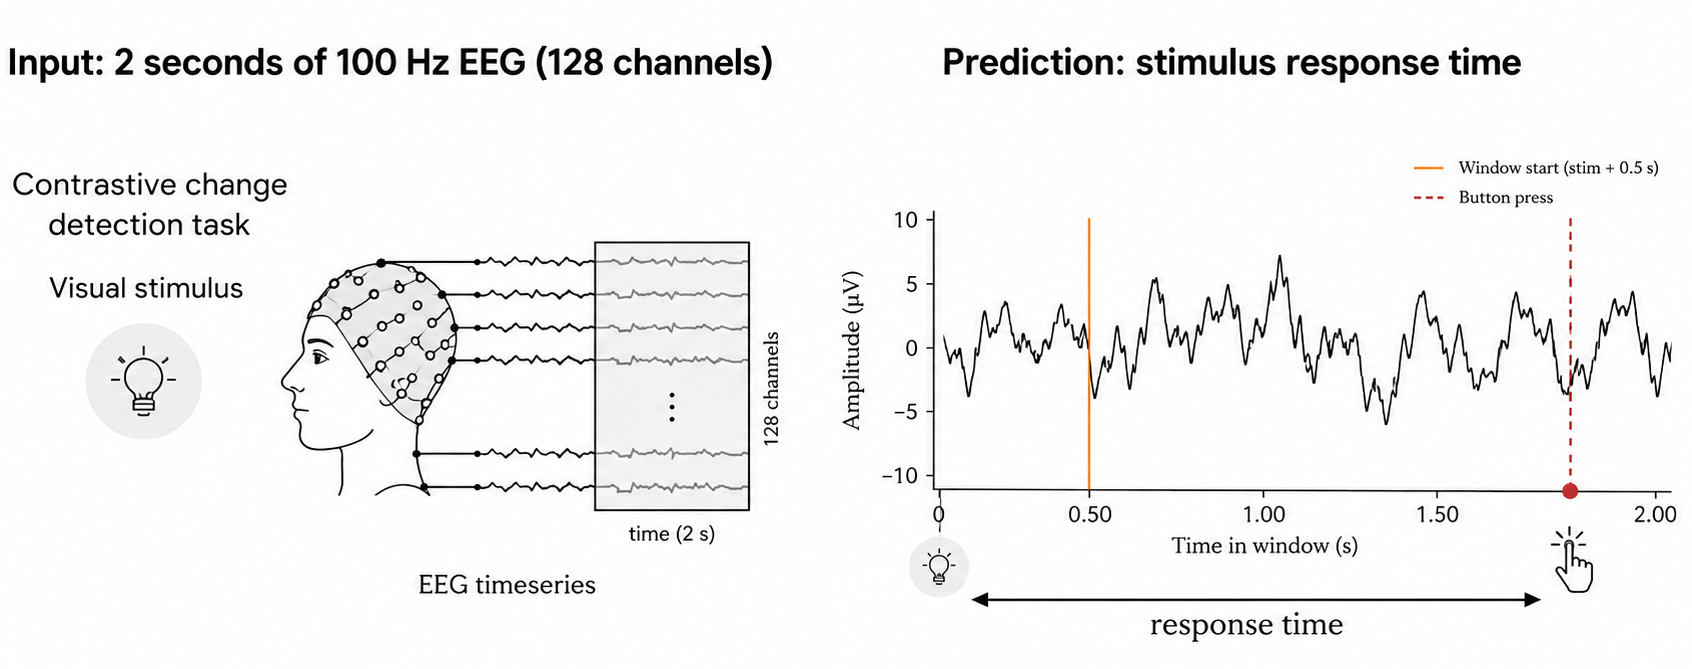
\includegraphics[width=0.9\linewidth]{img/challenge_task.png}
    \caption{Reaction-time prediction as event-time modeling. Each trial provides a 2~s stimulus-locked EEG window from the CCD paradigm (0.5--2.5~s after stimulus onset; 128 EEG channels at 100~Hz). The observed RT is represented as a smoothed distribution over post-stimulus time bins. The model predicts an event-time distribution, which is converted to a scalar RT prediction using a temperature-scaled soft-argmax readout.}
    \label{fig:tasks}
\end{figure}


\subsection{Preprocessing and Evaluation Protocol}

We evaluate models using a fixed split over HBN releases. Releases R1--R8 are used for fitting the base EEG models. Releases R9--R10 form the development partition used for checkpointing, calibration, protocol diagnostics, and stacking. When stacking is used, meta-model inputs on R9--R10 are generated using subject-disjoint out-of-fold predictions.

Release R11 serves as the labeled test release for final reporting. Model development, calibration, and selection are completed before R11 scoring. Main performance results are reported on R11 with subject-level bootstrap confidence intervals. The original hidden CodaBench evaluation from the EEG Foundation Challenge is reported separately in the Appendix as benchmark context.

For posterior-geometry analyses, we distinguish scalar RT evaluation from event-time support diagnostics. Scalar nRMSE is computed on all R11 trials, whereas posterior-shape summaries are restricted to trials whose observed RT is representable on the modeled event-time grid spanning 0.50--2.49~s from stimulus onset.

All neural models receive the same input normalization. For each 2~s trial window and each EEG channel, we subtract that channel's temporal mean within the window and divide by its temporal standard deviation within the same window. This transformation is computed independently within each input window and is applied identically across models.

Unless otherwise stated, training uses a fixed mild augmentation recipe. Channel dropout is applied with probability 0.25 and removes at most 30\% of channels. Temporal cutout is applied with probability 0.25 and masks a contiguous 10--50 sample interval, corresponding to at most 0.5~s in a 2~s, 100~Hz window. Gaussian noise is applied with probability 0.3 with standard deviation sampled as $0.01 + U(0,0.01)$. Mixup and stronger corruption recipes are excluded from the default protocol and treated only as appendix diagnostics.

\section{Methods}

\subsection{Scalar Regression Baselines}

\label{sec:baseline_regression}

We begin with baselines that treat the task as direct reaction-time regression: a stimulus-locked 2~s EEG crop $X \in \mathbb{R}^{C \times T}$ with $T=200$ samples (100~Hz) is mapped to a scalar RT.

Consistent with the low-SNR and distribution shift setting, we focus on lightweight backbones that are less prone to overfitting and enable extensive ablations, calibration, and ensembling.

All direct-regression baselines use the fixed 2~s input window, the per-window standardization described above, no mixup, batch size 128, patience 20, and the same release-separated train/development/holdout protocol. The default augmentation is the mild channel-dropout, temporal-cutout, and Gaussian-noise recipe described in the dataset protocol; stronger corruptions are retained only as appendix diagnostics.

For clarity, we use mechanism-level names in the manuscript. MSP-CNN denotes a multiscale segment-pooling CNN. It maps the full EEG window to scalar RT through temporal segment statistics and an MLP head. These models serve as reference points for isolating the effect of making temporal structure explicit in Section~\ref{sec:rt_segmentation}. In contrast to the segmentation formulation, direct scalar regression treats the window as a static input-output regression problem, without an explicit representation of response timing.

The main MSP-CNN regression backbone (Figure~\ref{fig:ch1_regression}) is a lightweight 1-D temporal ConvNet with:
(i) per-sample normalization to reduce cross-subject amplitude variation,
(ii) a learned channel-squeeze layer ($1\times1$ conv, 128$\rightarrow$96) that forms data-driven electrode mixtures,
and (iii) an EfficientNet-like temporal hierarchy with widening stages of residual depthwise-separable blocks
(96$\rightarrow$192$\rightarrow$384 channels) and anti-aliased temporal downsampling.
Coarse timing cues are retained using segment-wise statistical pooling: the time axis is split into 2 and 4 segments,
mean and max are computed per segment, and the resulting features are passed to a small MLP head.

External architectures are evaluated as supervised architectures trained from scratch under the same fixed preprocessing protocol. Pretrained weights are not used. The main tables report the wrapped/standardized variants because they receive the same per-window standardization as our models; unwrapped external runs are treated as sanity checks in the Appendix.

\begin{figure}[!t]
    \centering
    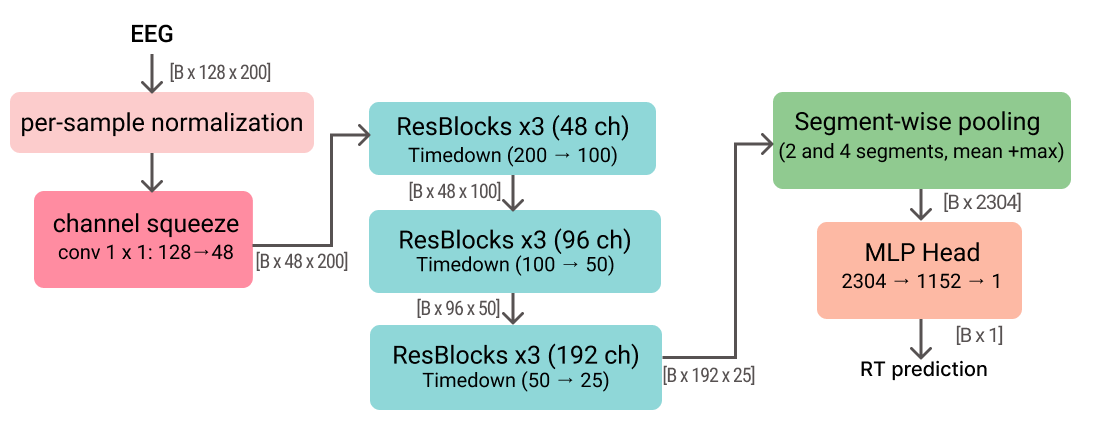
\includegraphics[width=\linewidth]{img/ch1/Ch1_regression.png}
    \caption{MSP-CNN direct RT regression baseline architecture. A lightweight 1-D temporal ConvNet maps a stimulus-locked 2~s EEG crop (128 channels, 100~Hz) to a scalar reaction-time prediction. Per-sample normalization and a learned $1\times1$ channel-squeeze layer (128$\rightarrow$96) are followed by residual depthwise-separable stages with anti-aliased temporal downsampling, segment-wise pooling (2 and 4 segments; mean+max), and an MLP head.}
    \label{fig:ch1_regression}
\end{figure}

\paragraph{Release-separated baseline comparison.}
Table~\ref{tab:r11_regression_baselines} reports direct-regression and external-backbone baselines under the release-separated protocol. The compact MSP-CNN and ETR-CNN models are the strongest direct-regression baselines under the fixed protocol. Wrapped external architectures are substantially better controlled than their unwrapped sanity-check counterparts, but remain behind the compact task-specific baselines on R11.

\begin{table}[!t]
\centering
\caption{Direct-regression and wrapped external backbone baselines under the release-separated protocol. R11 scores are reported with subject-bootstrap confidence intervals. Lower nRMSE is better.}
\label{tab:r11_regression_baselines}
\scriptsize
\setlength{\tabcolsep}{3pt}
\renewcommand{\arraystretch}{1.15}
\begin{tabularx}{\linewidth}{@{} >{\RaggedRight\arraybackslash}p{0.22\linewidth} Y c >{\RaggedRight\arraybackslash}p{0.27\linewidth} @{}}
\toprule
\textbf{Model} & \textbf{Role} & \textbf{Valid nRMSE} $\downarrow$ & \textbf{R11 nRMSE} $\downarrow$ \\
\midrule
MSP-CNN & compact scalar regression baseline & 0.933637 & 0.946269 [0.931609, 0.962943] \\
ETR-CNN & temporal-readout direct regression & 0.932577 & 0.945938 [0.930153, 0.963795] \\
ETR-CNN large & capacity ablation & 0.939308 & 0.951909 [0.936078, 0.969803] \\
TIDNet wrapped & strongest external supervised baseline in this comparison & 0.957974 & 0.959004 [0.948507, 0.970822] \\
EEGConformer wrapped & modern supervised transformer-style baseline & 0.957968 & 0.962802 [0.951634, 0.975382] \\
EEGNet wrapped & canonical compact EEG baseline & 0.957877 & 0.965041 [0.954684, 0.977111] \\
LaBraM wrapped & foundation-style architecture from scratch & 0.958254 & 0.965382 [0.952576, 0.979330] \\
Deep4Net wrapped & classical convolutional baseline & 0.955678 & 0.971619 [0.956680, 0.989067] \\
ATCNet wrapped & supervised conv/attention/TCN baseline & 0.970046 & 0.977366 [0.966497, 0.990685] \\
EEGPT wrapped & foundation-style architecture from scratch & 0.967140 & 0.978796 [0.969367, 0.990273] \\
\bottomrule
\end{tabularx}
\end{table}

Despite strong performance and fast training, direct regression does not explicitly represent the event-timing structure
of the task. Under heavier temporal jitter and cropping, optimization tended to over-focus on local waveform
micro-structure rather than learning \emph{when} the response-related event occurs. This limitation motivated the
segmentation reformulation in Section~\ref{sec:rt_segmentation}, which makes response timing explicit via an event-time
distribution.




\subsection{Temporal-Readout Regression}
\label{sec:rt_reg_zoo}


\begin{table}[!t]
\centering
\caption{Regression-style architecture families used before the event-time segmentation pivot. \emph{DS} = depthwise-separable. Current release-separated results are reported in Table~\ref{tab:r11_regression_baselines}.}
\label{tab:rt_regression_models}

\begingroup
\renewcommand{\baselinestretch}{1}\selectfont % prevent global double-spacing from enlarging table
\footnotesize                                % change to \scriptsize if still too tall
\setlength{\tabcolsep}{3pt}
\renewcommand{\arraystretch}{0.95}

% \begin{tabularx}{\linewidth}{@{} l Y l c c @{}}
\begin{tabularx}{\linewidth}{@{} 
p{0.14\linewidth} 
Y 
p{0.10\linewidth} 
c 
p{0.09\linewidth} 
@{}}

\toprule
\textbf{Model} & \textbf{Key design (high-level)} & \textbf{Temporal readout} & \textbf{Manuscript role} & \textbf{Size (MB)} \\

\midrule
MSP-CNN-S &
\textbf{Compact DS-residual encoder}\par
Shallow depth and small kernels emphasize local temporal motifs.
Strong temporal compression yields coarse features suited to pooling. &
Segment-stat pooling + MLP & compact MSP-CNN baseline & 4.95 \\

\addlinespace[0.3em]

MSP-CNN-L &
\textbf{Higher-capacity DS-residual encoder}\par
Wider/deeper stack and larger kernels increase temporal context and channel capacity.
Same coarse temporal hierarchy, but with stronger representational power. &
Segment-stat pooling + MLP & capacity ablation & 45.66 \\

\addlinespace[0.3em]

ETR-CNN-Dilated &
\textbf{Dilated DS-residual backbone}\par
Dilations expand receptive field while delaying temporal compression relative to MSP-CNN.
Designed to support distributional timing rather than coarse pooling. &
Temporal soft-argmax & ETR-CNN baseline & 49.24 \\

\addlinespace[0.3em]

Recurrent ETR-CNN (ACT) &
\textbf{Tied-weight recursive DS core}\par
Iterative refinement with step conditioning; adaptive computation via ACT halting.
Large effective depth at low parameter cost, paired with distributional timing. &
ACT temporal soft-argmax & exploratory readout variant & 1.67 \\

\bottomrule
\end{tabularx}

\endgroup

\end{table}


Temporal-readout regression is an intermediate baseline between scalar pooling and full event-time supervision. These models predict a distribution over time bins and read RT as an expectation, but the supervision remains scalar RT or an RT-derived readout loss rather than a full event-time posterior objective. Table~\ref{tab:rt_regression_models} summarizes representative regression-style architecture families; the release-separated performance comparison is reported in Table~\ref{tab:r11_regression_baselines}.

All baselines implement the same high-level pipeline: \emph{(a)} per-sample temporal standardization,
\emph{(b)} a learnable $1{\times}1$ channel-mixing projection ($C \!\rightarrow\! c_0$), and \emph{(c)} a lightweight
depthwise-separable residual convolutional backbone inspired by DS-ResNet style and MobileNet/Xception
\citep{howard2017mobilenets,chollet2017xception}. They differ mostly in how the final temporal feature map is converted into an RT estimate, that is, the \emph{temporal readout}.
In all cases, supervision remains scalar RT (or an RT-derived target) without explicit event-time labels; the temporal soft-argmax head is used only as a readout parameterization, not as event-time supervision.

We consider three temporal readout families. \textbf{Segment-stat pooling with an MLP} (MSP-CNN family) applies segmented mean and max
pooling over time to encode coarse early and late cues (conceptually similar to segment-based aggregation in TSN
\citep{wang2016tsn}), followed by an MLP regressor. \textbf{Temporal soft-argmax} (ETR-CNN) predicts a distribution
over time bins and reads RT as its expectation via a soft-argmax (coordinate-regression style) readout
\citep{nibali2018dsnt}. \textbf{ACT temporal soft-argmax} (recurrent ETR-CNN) refines the time distribution iteratively using tied
weights with adaptive computation time (ACT) style halting \citep{graves2016act} and FiLM conditioning \citep{perez2018film},
producing a halting-weighted mixture distribution before the same expectation readout. 
ETR-CNN additionally uses dilated convolutions to expand receptive field while delaying temporal compression relative to MSP-CNN \citep{yu2016dilated}.

\paragraph{Temporal-readout diagnostic.}
The release-separated comparison in Table~\ref{tab:r11_regression_baselines} shows that temporal readout alone provides only a marginal gain over scalar segment pooling: ETR-CNN reaches 0.945938 R11 nRMSE versus 0.946269 for MSP-CNN, while the larger ETR-CNN variant worsens to 0.951909. This indicates that parameterizing an expectation over time bins is not sufficient by itself. A temporal readout can be useful, but calibration under cross-subject and cross-release shift is not guaranteed by the readout alone, and the model is still not trained to match the geometry of an event-time posterior. These considerations motivate the segmentation formulation below, which makes response timing explicit via event-time supervision and distribution-matching losses.

\subsection{Event-Time Segmentation Framework}
\label{sec:rt_segmentation}

To make event timing explicit and to enable strong crop augmentation, RT prediction was reformulated as
\emph{temporal segmentation}: instead of regressing a scalar directly, we predict a distribution over time bins and read
out RT as its expectation (Figure~\ref{fig:ch1_pipeline}). Compared to distributional readouts used only as a final head, the key difference here is
that supervision is defined in time coordinates and shifted consistently under crop jitter, so augmentation preserves
the event-time target by construction. In practice, this produced a large performance gain and faster, more stable
convergence, while making crop augmentation safer because the supervision explicitly encodes \emph{where} the event occurs.
This is our RT instantiation of explicit temporal structure: behavior is modeled through event timing rather than static
regression.

\begin{figure}[!t]
    \centering
    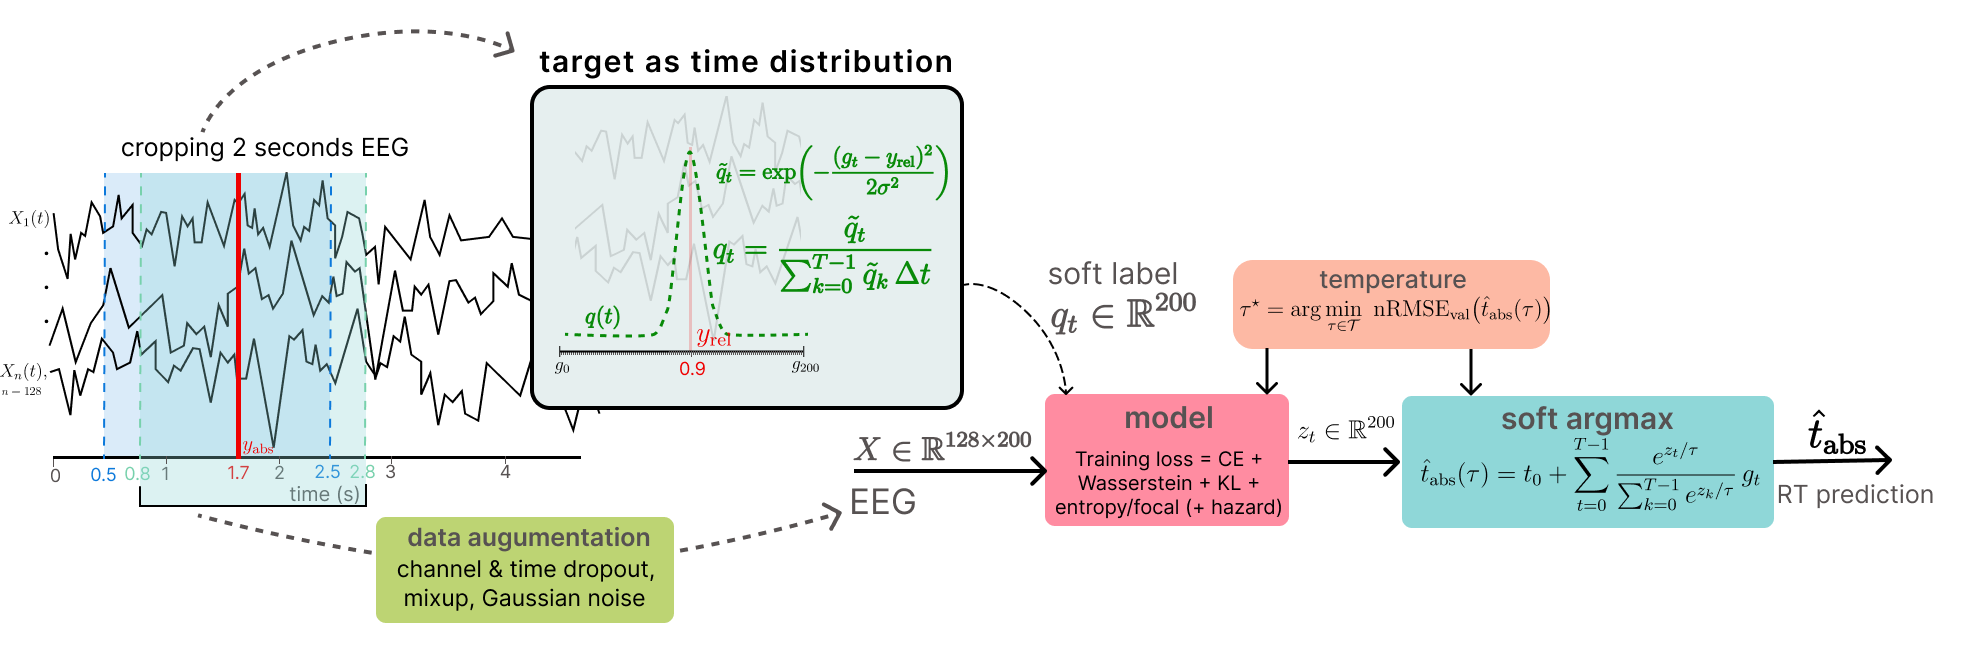
\includegraphics[width=\linewidth]{img/ch1/ch1_pipeline.png}
    \caption{Temporal segmentation pipeline for RT prediction.  For each trial we cache a longer stimulus-locked segment (4~s in our implementation) and sample a 2~s subwindow with start-time jitter for training; the RT label is shifted into the sampled window and a Gaussian soft target $q_t$ is formed. Per-time logits $z_t$ are produced by a 1-D segmentation model and are optimized with distribution-matching losses (e.g., soft-label CE, CDF-based Wasserstein-1, KL, and mild entropy penalty) or latent EventNLL objectives. The main readout is a temperature-scaled softmax posterior; hazard/survival readouts and alternate observation kernels are evaluated as compact extensions. RT is obtained by temperature-scaled soft-argmax, with $\tau^\star$ selected to minimize validation nRMSE.}
    \label{fig:ch1_pipeline}
\end{figure}

\paragraph{Notation and crop sampling.}
Let a 2~s crop be $X \in \mathbb{R}^{C\times T}$ with $\mathrm{sfreq}=100$~Hz, $T=200$ and $\Delta t=1/\mathrm{sfreq}$.
For training-time augmentation, we retain a longer stimulus-locked segment of length 4~s (0--4~s post-stimulus) and sample a 2~s subwindow from it, introducing temporal jitter while preserving trial identity. The crop start is clipped so that the labeled response remains inside the sampled 2~s window (label-preserving jitter). During validation and official inference, we always use the fixed stimulus-locked 2~s window with offset $t_0=0.5$~s (0.5--2.5~s), so that 
$t_{\mathrm{abs}} = t_0 + t_{\mathrm{rel}}$.

\paragraph{ETS-U-Net Architecture.}
\label{sec:ets_unet}

\begin{figure}[t]
    \centering
    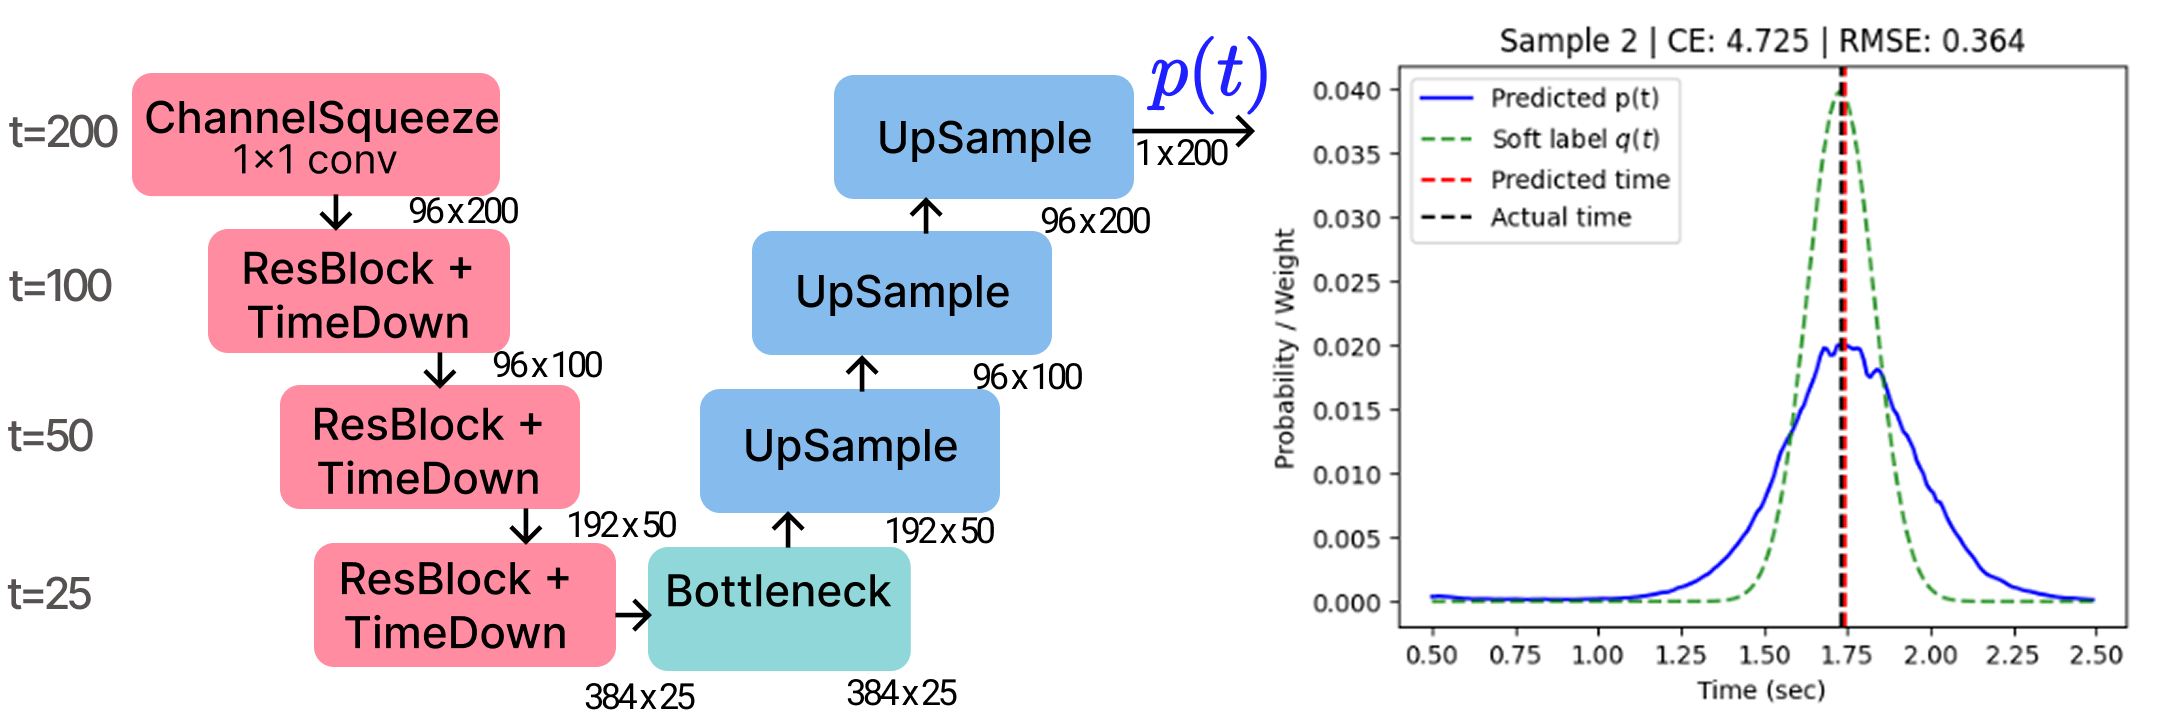
\includegraphics[width=0.9\linewidth]{img/ch1/Ch1_ets_unet_1.png}
    \caption{ETS-U-Net for RT segmentation. A lightweight 1-D U-Net maps a 2~s, 128-channel EEG crop to per-time logits
    and an event-time distribution $p(t)$. The encoder applies a $1\times1$ channel-squeeze layer followed by residual
    blocks with temporal downsampling (\texttt{TimeDown}); a bottleneck aggregates context, and the decoder upsamples with
    skip connections to recover time-resolved outputs. The right panel shows an example prediction $p(t)$ and Gaussian soft
    target $q(t)$, together with the resulting predicted vs.\ true response time.}
    \label{fig:ets_unet}
\end{figure}


The ETS-U-Net family is used to map a stimulus-locked EEG crop
$X\in\mathbb{R}^{C\times T}$ to per-time logits $z_{0:T-1}$ (Figure~\ref{fig:ets_unet}). All segmentation variants follow a 1-D U-Net style encoder-decoder with skip
connections for precise localization \citep{ronneberger2015unet}. The encoder progressively downsamples the temporal axis
to build multi-scale context, while the decoder upsamples and fuses encoder features to recover per-time outputs at the
original 200-sample resolution (internal down/up-sampling is used only to form multi-scale features). Each scale is refined
with lightweight residual blocks (ResNet-style skips) \citep{he2016resnet} built from depthwise-separable 1-D convolutions
for computational efficiency \citep{howard2017mobilenets,chollet2017xception}. To mitigate aliasing under temporal
decimation, downsampling applies a fixed depthwise smoothing filter followed by strided averaging (``blur-pool'' style)
\citep{zhang2019shiftinvariant}. A dilated bottleneck further enlarges the receptive field without additional downsampling
\citep{yu2016dilated}.



\textbf{Segmentation model zoo.} Table~\ref{tab:rt_seg_models} lists the variants used for ensembling/stacking.
ETS-U-Net-L/M/S share the same ETS-U-Net template and vary width and the number of residual refinement blocks per level.
Attention ETS-U-Net replaces the bottleneck with temporal multi-head self-attention (MHSA) \citep{vaswani2017attention} and uses
stochastic depth (DropPath) regularization \citep{huang2016stochasticdepth} to stabilize training at higher capacity.
EEG-Inception Segmentation replaces single-path temporal filtering with Inception-style multi-branch temporal kernels
\citep{szegedy2015going}, following the EEG-Inception design for ERP feature extraction \citep{santamaria2020eeginception}.
Finally, Factorized ETS-U-Net augments the channel-mixing front-end with factorized cross-channel interactions inspired by
Factorization Machines (FM) \citep{rendle2010fm}, optionally also injected within encoder stages to introduce a distinct
cross-channel inductive bias.


\begin{table}[t!]
\caption{Segmentation model variants used for reaction-time prediction. Each model outputs per-time logits and is trained under the same segmentation objective; architectural diversity is exploited for ensembling/stacking.}
\label{tab:rt_seg_models}
\small
\centering
\renewcommand{\arraystretch}{1.2}
\setlength{\tabcolsep}{4pt} % tighter column padding -> prevents overlap

% Make last two columns auto-wrap to fit the line
\begin{tabularx}{\linewidth}{@{}
  >{\RaggedRight\arraybackslash}p{0.20\linewidth}
  >{\RaggedRight\arraybackslash}p{0.16\linewidth}
  >{\RaggedRight\arraybackslash}X
  >{\RaggedRight\arraybackslash}X
@{}}
\hline
\textbf{Model} & \textbf{Architecture} & \textbf{Key features} & \textbf{Strengths} \\
\hline

ETS-U-Net-L (wide)
& ETS-U-Net
& wider encoder; depthwise-separable convs; 5 ResBlocks/level; dilated bottleneck
& highest capacity; captures complex local temporal patterns \\

ETS-U-Net-M
& ETS-U-Net
& moderate width; depthwise-separable convs; 5 ResBlocks/level; dilated bottleneck
& best single-model accuracy / efficiency tradeoff \\

ETS-U-Net-S
& ETS-U-Net
& lighter encoder; depthwise-separable convs; 3 ResBlocks/level; same bottleneck family
& fast, low-variance; complements deeper models \\

Attention ETS-U-Net (MHSA)
& Attention ETS-U-Net
& MHSA bottleneck (4 heads, depth=3); DropPath; positional depthwise conv
& captures long-range temporal dependencies \\

EEG-Inception Segmentation
& EEG-Inception 1D
& multi-branch temporal scales (0.5/0.25/0.125\,s) with feature fusion
& strong multi-scale feature extraction \\

Factorized ETS-U-Net
& Factorized ETS-U-Net
& FM-style cross-channel interactions at input; optional per-stage FM injection
& distinct cross-channel inductive bias \\
\hline
\end{tabularx}
\end{table}





Architectural diversity is introduced to improve ensembling and stacking. ETS-U-Net-L (wide) uses a wider encoder and
5 residual blocks per level, providing the highest capacity. ETS-U-Net-M retains the same depth (5 blocks/level) with a
more moderate width for a stronger accuracy--efficiency trade-off, while ETS-U-Net-S uses a lighter encoder
(3 blocks/level) and yields faster, lower-variance base learners. Long-range temporal interactions are emphasized in
Attention ETS-U-Net (MHSA) via a multi-head self-attention bottleneck. EEG-Inception Segmentation replaces single-path temporal filtering
with multi-branch kernels for multi-scale feature extraction. Finally, Factorized ETS-U-Net augments the standard channel-mixing
front-end with an FM-style factorized interaction module (optionally also injected within encoder stages), providing a
distinct cross-channel inductive bias. The post-hoc distribution-aware stacking procedure used for the secondary ensemble analysis is described in Appendix~\ref{sec:rt_stacking}.

\subsection{Soft-Label Distributional Supervision}

\paragraph{Soft target distribution.}
For a sampled crop, the ground-truth event time within the crop is represented as a relative time
$y_{\mathrm{rel}}\in[0,\mathrm{crop\_sec})$ with $\mathrm{crop\_sec}=2$.
A smooth segmentation label is constructed using a Gaussian kernel with bandwidth $\sigma$:
\begin{equation}
\label{eq:rt_soft_target}
\tilde q_t=\exp\left(-\frac{(g_t-y_{\mathrm{rel}})^2}{2\sigma^2}\right),\qquad
q_t=\frac{\tilde q_t}{\sum_{k=0}^{T-1}\tilde q_k},\qquad
\sum_{t=0}^{T-1} q_t=1.
\end{equation}
This smoothing stabilizes optimization while preserving temporal localization; in practice, $\sigma$ can be annealed
(start larger and decrease over training).

\paragraph{Model output and losses.}
A 1-D segmentation backbone produces logits $z_t$ for $t=0,\dots,T-1$, and a predicted
event-time distribution is obtained via temperature-scaled softmax,
\begin{equation}
\label{eq:rt_pred_dist}
p_t(\tau)=\frac{e^{z_t/\tau}}{\sum_{k=0}^{T-1} e^{z_k/\tau}}.
\end{equation}
The soft-label segmentation family is written as a weighted objective:
\begin{equation}
\label{eq:rt_loss}
\begin{aligned}
\mathcal{L}
&= \lambda_{\text{time}}\,\mathrm{RMSE}\big(\hat t_{\mathrm{rel}}(\tau), y_{\mathrm{rel}}\big)
 + \lambda_{\text{CE}}\,\mathrm{CE}\big(q, p(\tau)\big) \\
&\quad + \lambda_{W1}\,W_1\big(\mathrm{CDF}(q), \mathrm{CDF}(p(\tau))\big)
 + \lambda_{\text{KL}}\,D_{\mathrm{KL}}\big(q\|p(\tau)\big)
 - \lambda_{H}\,H\big(p(\tau)\big),
\end{aligned}
\end{equation}
where  
\begin{equation*}
\mathrm{CE}(q,p)=-\sum_{t=0}^{T-1} q_t \log p_t, \;
D_{\mathrm{KL}}(q\|p)=\sum_{t=0}^{T-1} q_t \log\frac{q_t}{p_t}, \;
H(p)=-\sum_{t=0}^{T-1} p_t \log p_t.
\end{equation*}
This expression defines an ablation family rather than a single mandatory loss cocktail. CE-only supervision sets the scalar time term to zero and asks the model to match a Gaussian soft event-time label. The hybrid objective combines CE with a soft-argmax time loss. The time-only ablation removes distributional matching while keeping the same readout, and the Wasserstein-only ablation tests whether a CDF-based geometry loss is sufficient on its own. The entropy, KL, focal, and related terms are best viewed as posterior-geometry controls rather than as the main contribution. We also evaluate a hazard-parameterized readout as an extension, mapping logits to a discrete-time survival process before forming the event-time posterior.

\paragraph{Release-separated segmentation comparison.}
Table~\ref{tab:r11_segmentation_losses} summarizes the event-time segmentation loss ablations, with the likelihood-family extensions defined in Section~\ref{sec:event_nll} included for comparison. The calibrated hybrid event-time segmentation model reaches 0.935573 nRMSE on R11, improving over the strongest direct-regression baseline. CE-only soft-label supervision is also strong. The Gaussian-mixture and hazard rows are compact EventNLL-family extensions: the former changes the observation kernel, while the latter changes the event-time posterior parameterization. This is the central empirical step in the narrative: once RT is represented as an event-time posterior, distributional supervision over time becomes more useful than treating RT as a scalar window label.

\begin{figure}[!t]
    \centering
    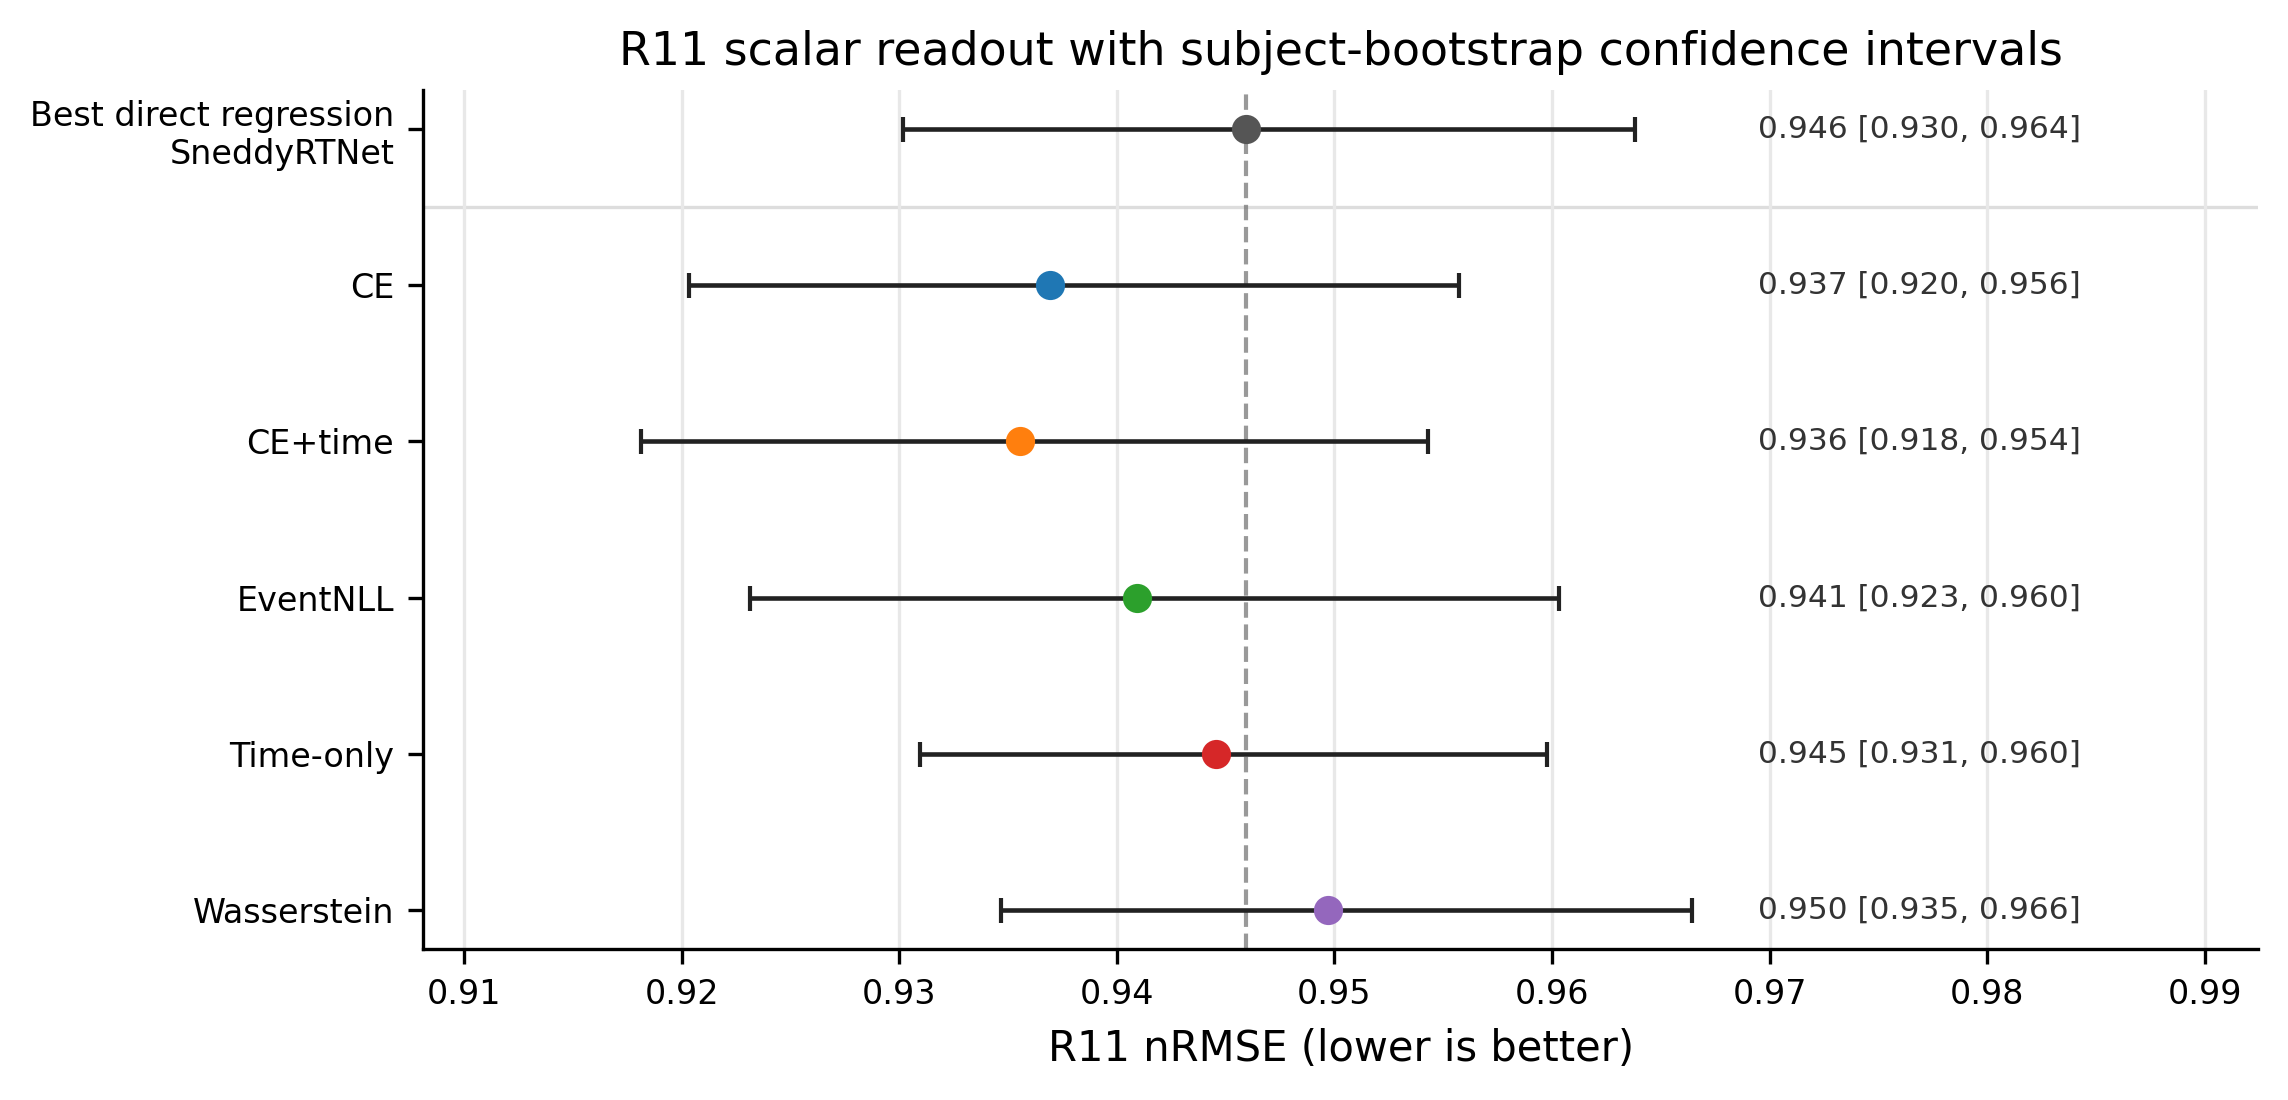
\includegraphics[width=\linewidth]{img/ch1/r11_performance_forest_calibrated.png}
    \caption{R11 scalar readout performance with subject-bootstrap confidence intervals. The dashed vertical line marks the strongest direct-regression baseline. Several event-time losses improve scalar nRMSE while remaining close enough to motivate posterior-level analysis rather than ranking losses only by point-prediction error.}
    \label{fig:r11_performance_forest}
\end{figure}

\begin{table}[!t]
\centering
\caption{Completed event-time segmentation loss ablations under the release-separated protocol. ``Cal.'' denotes post-hoc temperature selection on R9-R10 and one-shot application to R11.}
\label{tab:r11_segmentation_losses}
\scriptsize
\setlength{\tabcolsep}{3pt}
\renewcommand{\arraystretch}{1.15}
\begin{tabularx}{\linewidth}{@{} >{\RaggedRight\arraybackslash}p{0.17\linewidth} Y c c >{\RaggedRight\arraybackslash}p{0.27\linewidth} @{}}
\toprule
\textbf{Run} & \textbf{Objective} & $\boldsymbol{\tau}$ & \textbf{Valid nRMSE} $\downarrow$ & \textbf{R11 nRMSE} $\downarrow$ \\
\midrule
CE only, base & soft-label event-time CE & 0.65 & 0.922529 & 0.938738 [0.921696, 0.958015] \\
CE only, cal. & soft-label event-time CE & 0.70 & 0.922277 & 0.936942 [0.920329, 0.955704] \\
Hybrid, base & soft-label CE + soft-argmax time loss & 0.65 & 0.925601 & 0.940006 [0.921243, 0.960020] \\
Hybrid, cal. & soft-label CE + soft-argmax time loss & 0.80 & 0.924544 & 0.935573 [0.918136, 0.954309] \\
Event NLL, cal. & continuous latent event-time likelihood & 0.70 & 0.923619 & 0.940947 [0.923160, 0.960322] \\
Gaussian mixture NLL, cal. & two-scale EventNLL observation kernel & 0.75 & 0.921676 & 0.939267 [0.921864, 0.958291] \\
Hazard EventNLL & hazard-parameterized event-time posterior & 0.65 & 0.924318 & 0.937332 [0.920594, 0.955704] \\
Time only, cal. & soft-argmax scalar time loss only & 0.85 & 0.935298 & 0.944578 [0.930935, 0.959775] \\
Wasserstein only, cal. & event-time CDF distance only & 2.95 & 0.936941 & 0.949716 [0.934666, 0.966443] \\
\bottomrule
\end{tabularx}
\end{table}

\paragraph{Objective ablations.}
The loss ablations separate the value of the temporal readout from the value of distributional supervision. The time-only model directly optimizes soft-argmax error but removes distribution matching; it is weaker than CE-only and hybrid segmentation. The Wasserstein-only run is a useful negative control: not every distributional distance recovers the gain. CE, CE+time, and EventNLL remain in the same performance band, supporting the view that the main gain comes from the event-time formulation rather than from a single hand-tuned loss. The hazard EventNLL result further shows that the formulation is not tied to a categorical softmax readout: a survival-style posterior reaches the same scalar-performance regime while preserving the event-time likelihood view.

\paragraph{Seed robustness.}
To test whether the main comparison depends on a favorable random initialization, we repeated selected core recipes over five seeds (2025--2029). This analysis is a reliability check rather than a new model-selection stage: it focuses on the strongest temporal-readout regression baseline, the strongest wrapped external baseline, the two main distributional event-time objectives, and the time-only segmentation control.

Table~\ref{tab:seed_robustness} shows that the central event-time supervision gap is stable. CE and EventNLL segmentation remain about 0.010--0.011 R11 nRMSE better than the repeated ETR-CNN scalar baseline on average. In contrast, the time-only segmentation control is much closer to ETR-CNN, supporting the interpretation that the gain comes from distributional event-time supervision rather than only from a U-Net backbone or soft-argmax readout. The optional repeated TIDNet baseline also remains weaker than both ETR-CNN and the event-time segmentation variants.

\begin{table}[!t]
\centering
\caption{Five-seed robustness summary for selected core models. Values are mean $\pm$ sample standard deviation over seeds 2025--2029; R11 range is min--max across seeds. Posterior scores are reported only for event-time segmentation runs. Lower is better for all metrics.}
\label{tab:seed_robustness}
\scriptsize
\setlength{\tabcolsep}{3pt}
\renewcommand{\arraystretch}{1.12}
\resizebox{\linewidth}{!}{%
\begin{tabular}{@{} l l c c c c c @{}}
\toprule
\textbf{Model} & \textbf{Role} & \textbf{Valid nRMSE} $\downarrow$ & \textbf{R11 nRMSE} $\downarrow$ & \textbf{R11 range} & \textbf{Posterior CRPS} $\downarrow$ & \textbf{Fixed NLL} $\downarrow$ \\
\midrule
ETR-CNN & temporal-readout scalar baseline & 0.9359 $\pm$ 0.0031 & 0.9495 $\pm$ 0.0048 & 0.9451--0.9570 & -- & -- \\
TIDNet wrapped & strongest wrapped external baseline & 0.9546 $\pm$ 0.0014 & 0.9614 $\pm$ 0.0046 & 0.9547--0.9656 & -- & -- \\
ETS-U-Net CE & soft-label event-time CE & 0.9209 $\pm$ 0.0024 & 0.9384 $\pm$ 0.0021 & 0.9352--0.9407 & 0.1927 $\pm$ 0.0007 & 0.3062 $\pm$ 0.0086 \\
ETS-U-Net EventNLL & latent event-time likelihood & 0.9242 $\pm$ 0.0024 & 0.9391 $\pm$ 0.0045 & 0.9318--0.9439 & 0.2011 $\pm$ 0.0019 & 0.1523 $\pm$ 0.0133 \\
ETS-U-Net time-only & soft-argmax time loss control & 0.9371 $\pm$ 0.0020 & 0.9473 $\pm$ 0.0021 & 0.9447--0.9496 & 0.2040 $\pm$ 0.0020 & 0.3878 $\pm$ 0.0268 \\
\bottomrule
\end{tabular}%
}
\end{table}

\subsection{Latent Event-Time Likelihood}
\label{sec:event_nll}

As a probabilistic alternative to soft Gaussian-label supervision, we also evaluate a latent event-time likelihood. The temporal softmax defines a posterior over latent event bins, and the observed scalar RT is modeled as a noisy realization of the latent event time:
\begin{equation}
\label{eq:event_nll}
p(y\mid X)
= \sum_{t=0}^{T-1} p_t(X)\,
\mathcal{N}\!\left(y;\,t_0 + g_t,\,\sigma_y^2\right),
\qquad
\mathcal{L}_{\mathrm{EventNLL}} = -\log p(y\mid X).
\end{equation}
This objective keeps the same event-time interpretation but replaces the artificial target mask $q_t$ with a marginal likelihood over latent response-relevant event times. We therefore present EventNLL primarily as a more principled latent-variable objective, not as the scalar-NRMSE winner among the evaluated losses.

\paragraph{Observation-kernel and hazard extensions.}
The EventNLL formulation separates the latent event-time posterior $p_t(X)$ from the observation model $K(y\mid t)$. The default model uses a single Gaussian observation kernel, but we also evaluate a two-scale Gaussian mixture,
\begin{equation}
\label{eq:event_nll_mixture_kernel}
K(y\mid t)=(1-\alpha)\,\mathcal{N}(y;t_0+g_t,\sigma_{\mathrm{narrow}}^2)
+\alpha\,\mathcal{N}(y;t_0+g_t,\sigma_{\mathrm{wide}}^2),
\end{equation}
which keeps most probability mass in a narrow timing error while allowing a wider tail for occasional noisy RT observations. In the completed run, $\sigma_{\mathrm{narrow}}=0.10$~s, $\sigma_{\mathrm{wide}}=0.35$~s, and $\alpha=0.10$.

As a readout extension, we also evaluate a hazard/survival parameterization. Instead of using logits only as unconstrained softmax scores, each temporal logit defines a conditional event probability
\begin{equation}
\label{eq:hazard_readout}
h_t=\sigma(z_t/\tau),\qquad
p_t^{\mathrm{haz}} \propto h_t\prod_{k<t}(1-h_k),
\end{equation}
with the resulting event-bin probabilities normalized over the represented window. This keeps the same event-time likelihood in Eq.~\ref{eq:event_nll}, but changes the posterior parameterization from a categorical softmax to a discrete-time survival process. We treat this as a paper-facing extension because it tests whether the event-time formulation is tied to one softmax implementation.

\paragraph{Likelihood-family comparison.}
The EventNLL rows in Table~\ref{tab:r11_segmentation_losses} show that the event-time NLL run nearly matches CE-only and hybrid segmentation without requiring a hand-weighted CE+time objective. We therefore present it as a principled latent-variable likelihood rather than as a claim of best scalar nRMSE. The Gaussian-mixture kernel improves the EventNLL-family scalar readout relative to the fixed Gaussian kernel, while the hazard EventNLL extension reaches CE-level R11 performance without reverting to scalar regression. The posterior-geometry analysis in Table~\ref{tab:posterior_geometry_metrics} further shows that EventNLL produces a much narrower posterior than CE or CE+time and places more mass near the target, but it also under-covers nominal central intervals. This makes it scientifically useful: it reveals that similar scalar errors can correspond to different posterior geometries.

\subsection{Posterior Geometry and Readout Temperature Tuning}

The posterior view makes geometric properties of the predicted distribution directly inspectable. CDF-based distances penalize temporal displacement of probability mass, entropy and variance summarize posterior sharpness, and quantiles expose asymmetric uncertainty around the predicted response time. These summaries are useful for diagnosis and for downstream stacking.

When used, explicit posterior regularization can be written generically as
\begin{equation}
\label{eq:posterior_regularized_objective}
\mathcal{L} = \mathcal{L}_{\mathrm{event}} + \lambda R\!\left(p(t\mid X)\right),
\end{equation}
where $R$ may target entropy, variance, tail mass, or other posterior-shape statistics. In this manuscript we treat such terms as analysis and control of posterior geometry unless a clean ablation has been completed.

\paragraph{Inference and temperature tuning.}
The relative event time is estimated by expectation (soft-argmax),
\begin{equation}
\label{eq:rt_soft_argmax}
\hat t_{\mathrm{rel}}(\tau)=\sum_{t=0}^{T-1} p_t(\tau)\, g_t,
\qquad
\hat t_{\mathrm{abs}}(\tau)=t_0+\hat t_{\mathrm{rel}}(\tau),
\end{equation}
where $g_t=t\,\Delta t$ denotes the discrete time grid. Under squared error, the Bayes-optimal point estimate is the
conditional mean; accordingly, reading out RT by $\mathbb{E}_{p(t)}[g]$ aligns naturally with the nRMSE objective (RMSE
up to a constant normalization).

In practice, different training choices (loss weighting, augmentation strength, and checkpoint selection) produced
time-distributions with markedly different sharpness and entropy: some models generated very peaked $p(t)$ while others
were systematically more diffuse. This creates a confidence-scale mismatch, where naive averaging (or stacking without
temperature-scaled inputs) can underweight accurate but underconfident models and overweight overconfident ones.

We therefore use post-hoc temperature scaling \citep{guo2017calibration} to tune the softness of $p(t)$, improving the
readout and making confidence profiles more comparable across losses and models.
Temperature is selected by validation tuning for each base model $m$:

\begin{equation}
\label{eq:rt_tau_tuning}
\tau_m^\star = \arg\min_{\tau\in\mathcal{T}_{\text{cal}}}
\ \mathrm{nRMSE}_{\text{val}}\big(\hat t_{\mathrm{abs}}^{(m)}(\tau)\big).
\end{equation}

Under the release-separated protocol, $\mathcal{T}_{\text{cal}}$ is selected on the R9-R10 development split and applied unchanged to R11.

Because confidence scales differ across objectives and architectures, temperature is treated as a posterior-geometry
control selected on development data rather than as a separate model-selection signal.

\paragraph{Posterior geometry and interval coverage.}
The scalar comparisons above compare models through the posterior mean, but the event-time formulation produces a full distribution over response latencies. Two losses can therefore have similar nRMSE while assigning probability mass very differently over time. We analyze this posterior geometry to ask whether the scalar prediction is supported by a localized temporal event distribution, whether the posterior is overly diffuse or overly concentrated, and whether nominal posterior intervals have meaningful empirical coverage.

For this analysis, the softmax temperature is selected on R9--R10 to minimize scalar nRMSE of the posterior-mean readout. Thus, we treat temperature selection as readout-temperature tuning rather than as full probabilistic calibration. After this readout tuning, we evaluate the learned event-time posterior itself: whether its mass is near the observed RT, whether the posterior mean agrees with the posterior mode, and whether nominal posterior intervals contain the true RT at the expected rate.

Figure~\ref{fig:posterior_raster_main} provides a trial-sorted view of these posteriors before reducing them to summary metrics. It shows how each loss distributes probability mass across the represented RT range, making posterior width, target alignment, and loss-specific confidence patterns visible at the dataset level.

Table~\ref{tab:posterior_geometry_metrics} uses four groups of metrics. First, scalar nRMSE and MAE measure the posterior-mean RT prediction. Second, CRPS and fixed-kernel EventNLL score the full posterior distribution; lower values indicate better distributional predictions. The fixed-kernel EventNLL uses the same Gaussian observation kernel for all models, so it evaluates the predicted event-time distribution under a common likelihood score rather than under each model's own training loss. Third, Width80, Mass $\pm$150 ms, and mode-mean gap describe posterior geometry: Width80 is the median width of the nominal 80\% central posterior interval, Mass $\pm$150 ms is the posterior probability assigned within 150 ms of the observed RT, and mode-mean gap measures disagreement between the posterior peak and the posterior mean used for scalar readout. Finally, Coverage80 and Coverage MAE summarize interval coverage. Coverage80 is the empirical coverage of the nominal 80\% central interval, whose calibrated target is 0.80. Coverage MAE is the mean absolute difference between empirical and nominal coverage over central intervals $\{50\%,60\%,70\%,80\%,90\%\}$.

\begin{figure}[!t]
    \centering
    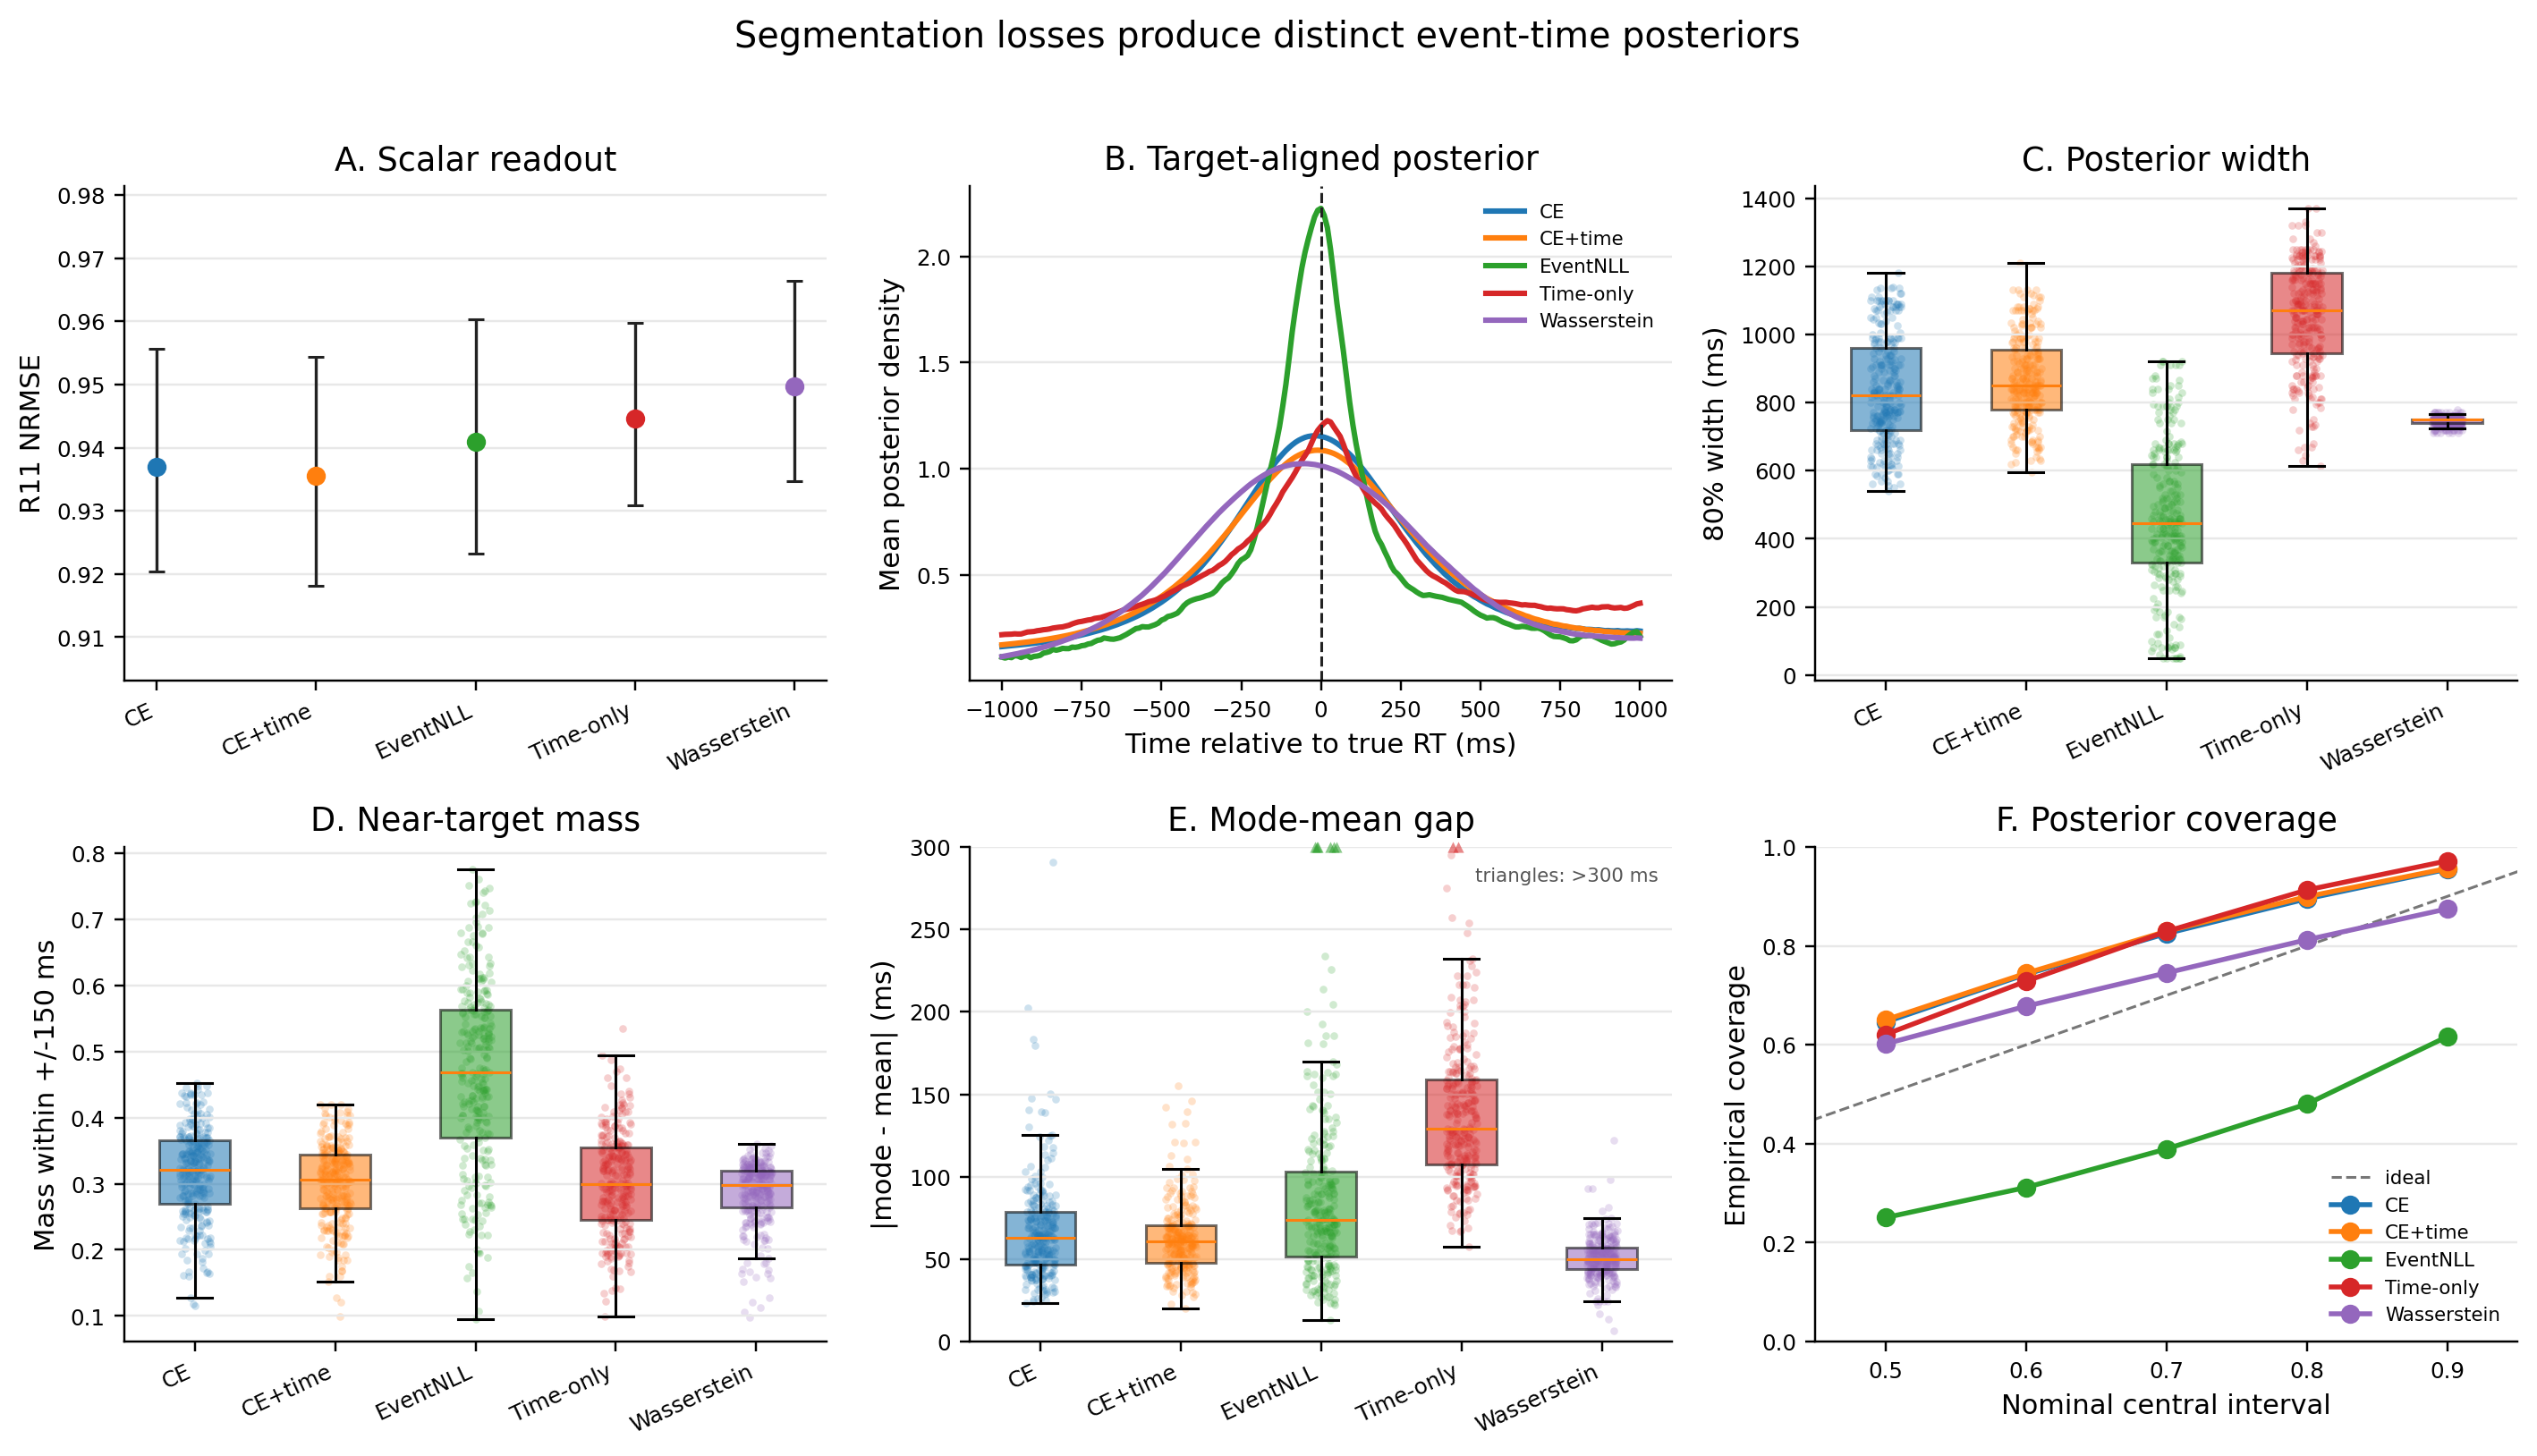
\includegraphics[width=\linewidth]{img/ch1/posterior_geometry_main_calibrated.png}
    \caption{Posterior geometry differs across event-time losses even when scalar nRMSE is similar. Panel A reports R11 scalar readout after selecting the softmax temperature on R9--R10 to minimize nRMSE. Panel B aligns predicted posteriors to the true RT. Panels C--E summarize posterior width, near-target mass, and mode-mean disagreement. Panel F compares empirical coverage of central posterior intervals; the diagonal is ideal interval coverage.}
    \label{fig:posterior_geometry_main}
\end{figure}

\begin{figure}[!t]
    \centering
    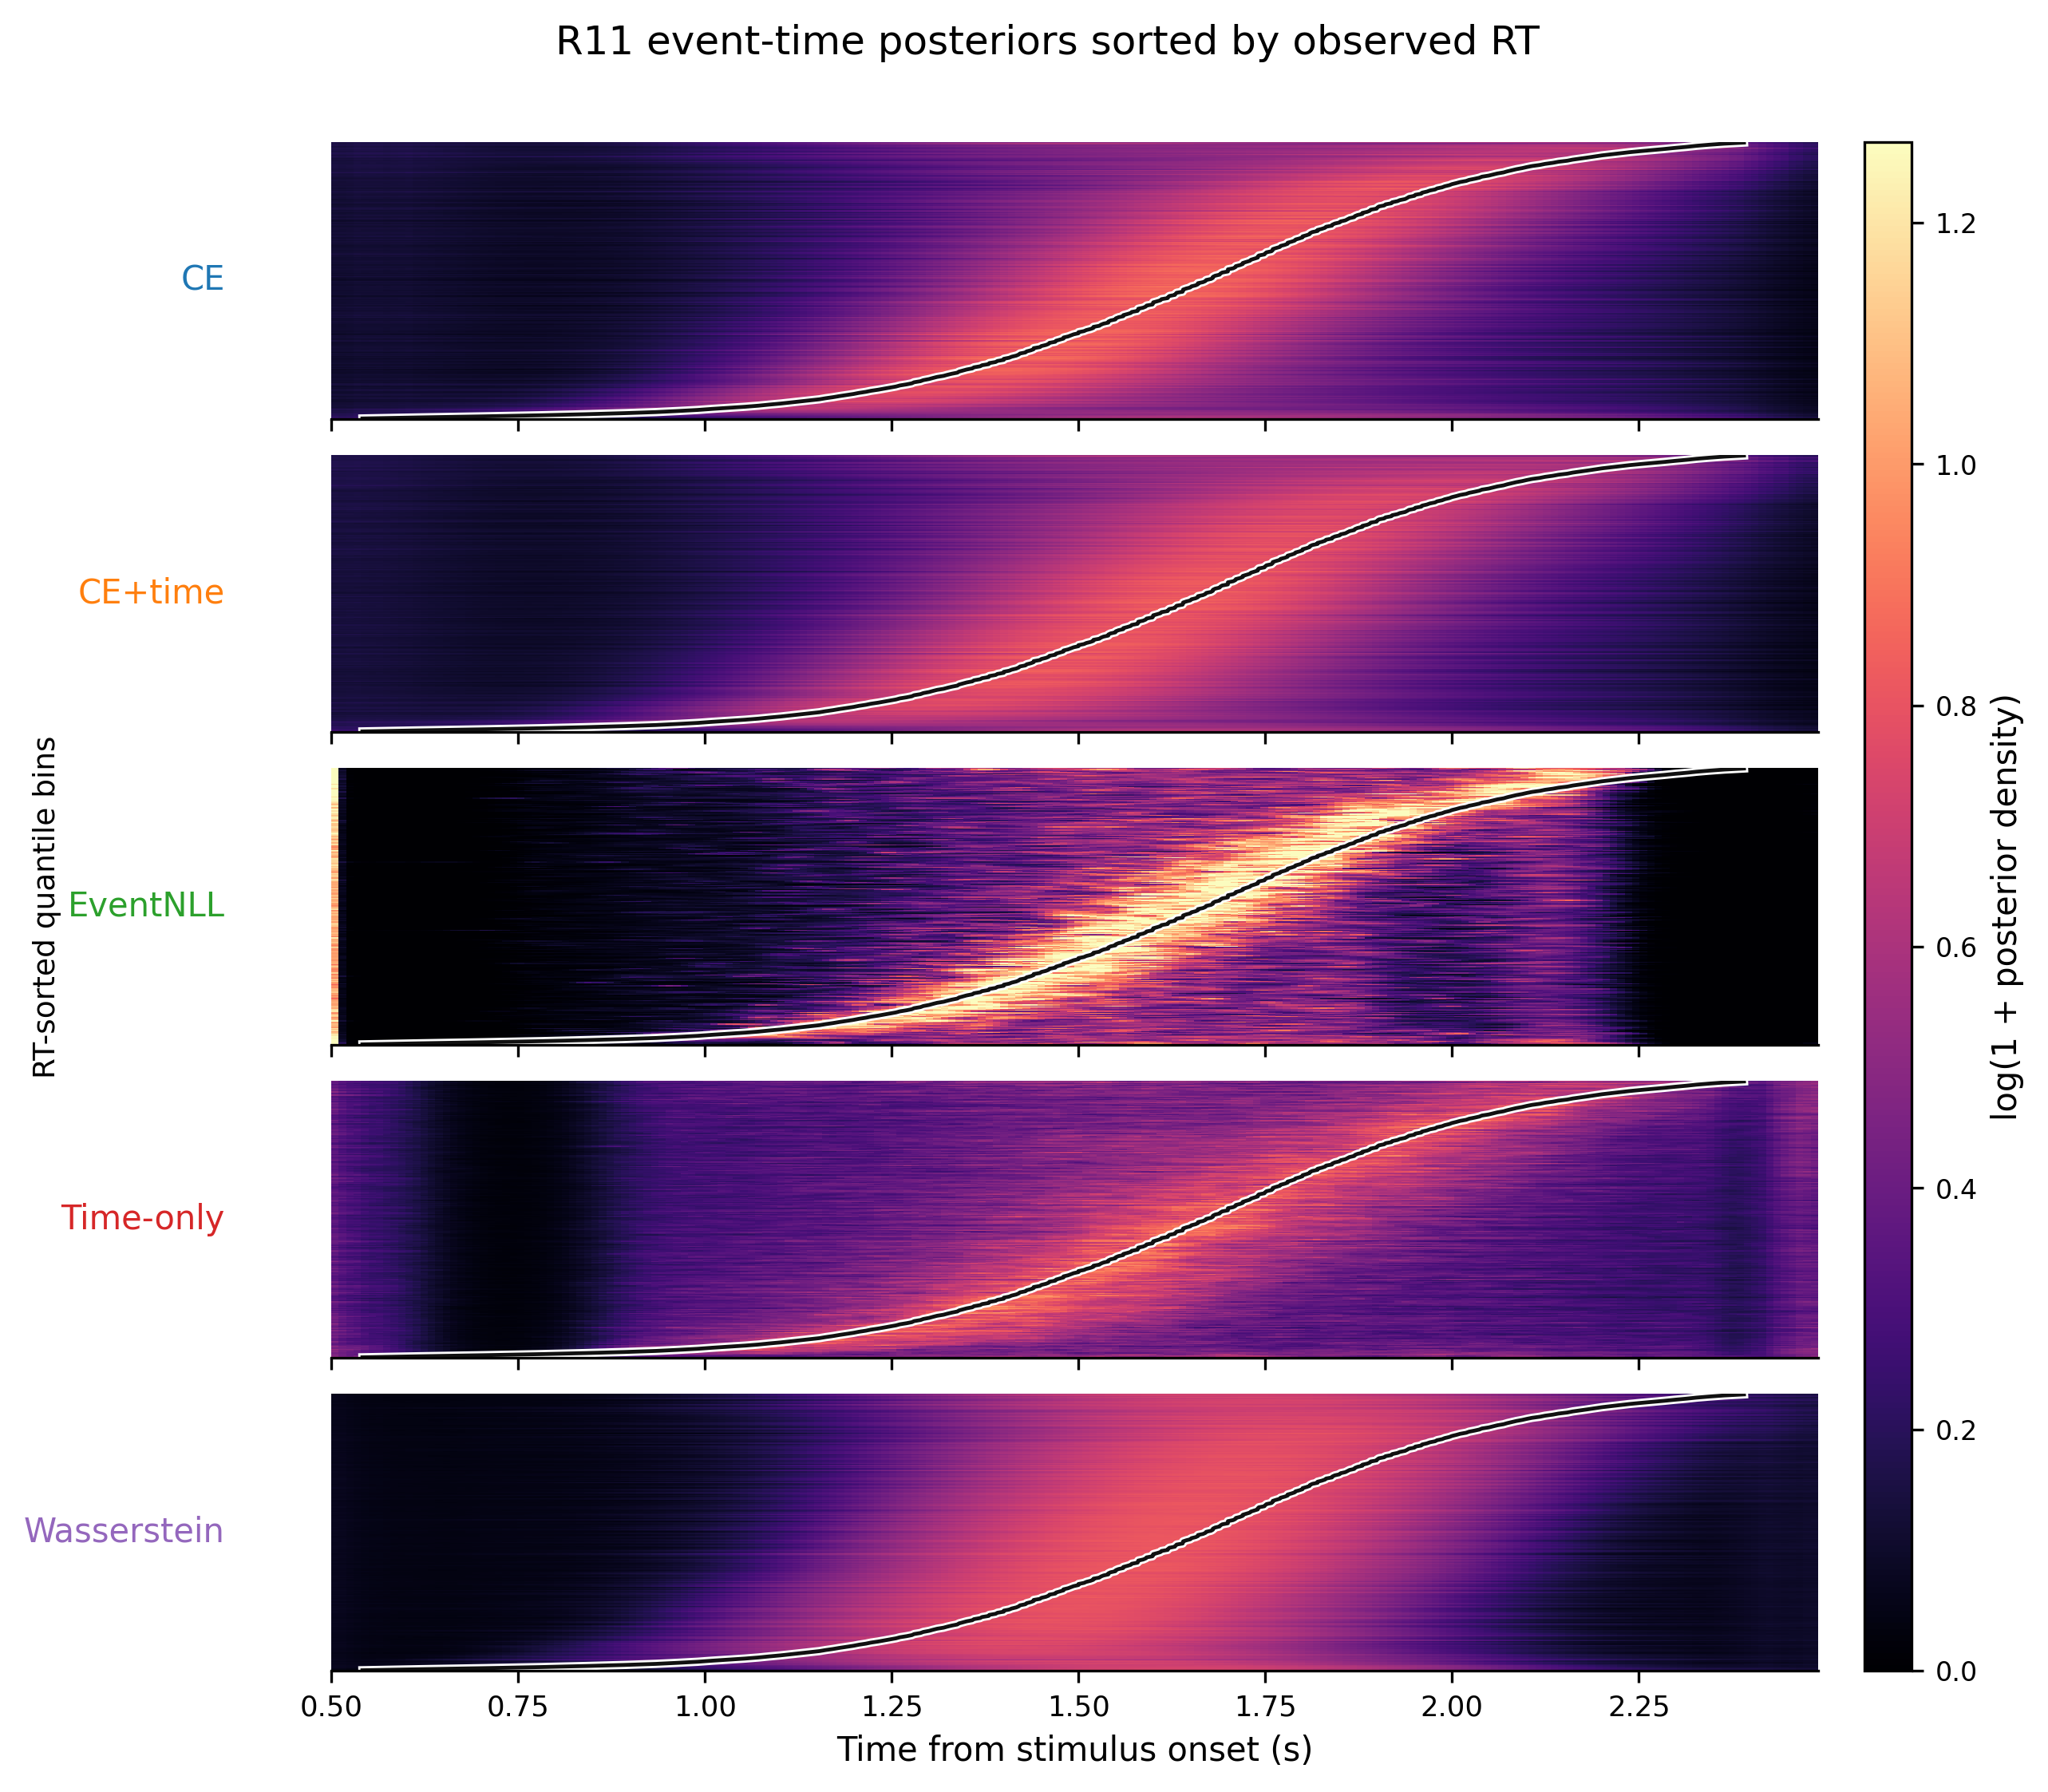
\includegraphics[width=\linewidth]{img/ch1/trial_sorted_posterior_raster_calibrated.png}
    \caption{Trial-sorted event-time posterior maps on R11 for matched segmentation losses. Rows are quantile bins of representable R11 trials sorted by observed RT; the x-axis is time from stimulus onset; color shows log-transformed posterior density averaged within each bin. The black curve marks the mean observed RT in each bin.}
    \label{fig:posterior_raster_main}
\end{figure}

\begin{table}[!t]
\centering
\caption{Quantitative posterior geometry on R11 for matched event-time segmentation losses. Metrics are defined in the text. CRPS is reported in milliseconds. Fixed-kernel EventNLL uses a common Gaussian observation kernel for all models ($\sigma=0.15$~s). For Coverage80, values closer to 0.80 indicate better nominal 80\% interval coverage; for Coverage MAE, lower is better.}
\label{tab:posterior_geometry_metrics}
\scriptsize
\setlength{\tabcolsep}{3pt}
\renewcommand{\arraystretch}{1.12}
\resizebox{\linewidth}{!}{%
\begin{tabular}{@{} l c c c c c c c c c @{}}
\toprule
\textbf{Model} & \textbf{nRMSE} & \textbf{MAE ms} & \textbf{CRPS ms} & \textbf{Fixed NLL} & \textbf{Width80 ms} & \textbf{Mass $\pm$150 ms} & \textbf{Mode-mean gap ms} & \textbf{Coverage80} & \textbf{Coverage MAE} \\
\midrule
CE & 0.937 & 216 & 155 & 0.115 & 820 & 0.328 & 57 & 0.895 & 0.113 \\
CE+time & 0.936 & 219 & 157 & 0.144 & 860 & 0.311 & 57 & 0.899 & 0.116 \\
EventNLL & 0.941 & 216 & 162 & -0.027 & 450 & 0.487 & 72 & 0.480 & 0.290 \\
Time-only & 0.945 & 228 & 167 & 0.203 & 1070 & 0.311 & 129 & 0.913 & 0.113 \\
Wasserstein & 0.950 & 222 & 165 & 0.219 & 740 & 0.296 & 50 & 0.812 & 0.053 \\
\bottomrule
\end{tabular}%
}
\end{table}

These metrics show that the losses induce different output semantics. CE+time and CE give the strongest scalar readouts, but their nominal 80\% intervals cover about 90\% of trials, indicating conservative over-coverage. EventNLL is not well calibrated as an uncertainty posterior: its nominal 80\% interval covers only 48\% of trials. Its value is instead localization-like concentration, with the narrowest Width80, the highest near-target mass, and the best fixed-kernel EventNLL score. Wasserstein has the smallest Coverage MAE and a Coverage80 value closest to 0.80, but this comes with weaker scalar nRMSE and lower near-target mass. Thus, posterior geometry reveals a trade-off among scalar accuracy, target concentration, and interval coverage that is hidden by nRMSE alone.

\paragraph{Secondary ensemble use of posterior features.}
The same posterior summaries can also serve as post-hoc ensemble features, but we treat this as a secondary analysis rather than as a main release-separated claim. The single-model R11 comparisons above are intentionally reported without stacking, so that the main evidence isolates the event-time objective, scalar readout, posterior geometry, and the shifted-crop diagnostic below. The stacker construction is described in Appendix~\ref{sec:rt_stacking}; in the original hidden-release CodaBench evaluation (Appendix Table~\ref{tab:appendix_codabench}), gradient boosting stacking achieved 0.91394 hidden nRMSE, compared with 0.92334 for the best single model, 0.91840 for manual blending, and 0.91539 for Ridge stacking. This supports posterior-derived meta-features as an ensemble calibration layer while keeping the paper's main claims tied to single-model release-separated analyses.

\subsection{Shifted-Crop Localization Diagnostic}

The posterior analyses above show that event-time losses produce different probability geometries, but they do not by themselves prove that a model has learned a within-crop event localizer. A fixed stimulus-locked window can still permit shortcut behavior: a model may predict trial difficulty, subject-level slowness, or stimulus-locked response tendency without moving its prediction when the crop is shifted. We therefore introduced a shifted-crop diagnostic on R11. For each trial, we used a 5~s EEG window and evaluated the same trained model on 2~s crops starting at $s\in\{0.2,0.3,\dots,0.8\}$~s. The reference crop is $s=0.5$~s, matching the training and main inference protocol. To avoid target-censoring effects, this analysis uses the common-inside subset where RT remains inside all shifted crops ($0.8\leq \mathrm{RT}\leq 2.2$~s; 14{,}183 trials).

If the model truly localizes the response-relevant event within the crop, shifting the crop start by $\Delta s$ should move the predicted crop-relative event time by approximately $-\Delta s$, giving a raw shift slope near $-1$. A crop-invariant scalar regressor should instead have a slope near 0. Table~\ref{tab:shifted_crop_diagnostic} shows that the event-time segmentation models preserve or improve reference-crop accuracy and move in a more localizer-like direction than the best scalar regressor. EventNLL reaches a raw shift slope of $-0.292$ [95\% CI: $-0.311$, $-0.272$], compared with $-0.253$ [$-0.270$, $-0.235$] for ETR-CNN and $-0.172$ on average across regression baselines. The fraction of localizer-like trials also increases from 10.1\% for ETR-CNN to 14.8\% for CE and 15.9\% for EventNLL.

This result should be interpreted as evidence for a representational shift, not as solved shift equivariance. The segmentation models remain far from the ideal slope of $-1$, indicating that fixed-window training still mixes event localization with scalar response-tendency shortcuts. That limitation is useful: it identifies shift-augmented, crop-relative event-time training as the natural next step if the goal is a stronger trial-wise neural event localizer.

\begin{table}[!t]
\centering
\caption{Shifted-crop diagnostic on the R11 common-inside subset. The ideal within-crop event localizer has raw shift slope $-1$; a crop-invariant scalar shortcut has slope 0. Reference nRMSE is computed at the standard $s=0.5$~s crop.}
\label{tab:shifted_crop_diagnostic}
\scriptsize
\setlength{\tabcolsep}{3pt}
\renewcommand{\arraystretch}{1.12}
\resizebox{\linewidth}{!}{%
\begin{tabular}{@{} l c c c c c c @{}}
\toprule
\textbf{Model} & \textbf{Ref nRMSE} $\downarrow$ & \textbf{Ref MAE, s} $\downarrow$ & \textbf{Worst $\Delta$ nRMSE} & \textbf{Raw shift slope} & \textbf{Localizer-like trials} & \textbf{Invariant-like trials} \\
\midrule
ETR-CNN & 0.874 & 0.206 [0.199, 0.215] & 0.174 & $-0.253$ [$-0.270$, $-0.235$] & 10.1\% [9.0, 11.1] & 34.5\% \\
ETS-U-Net CE & 0.856 & 0.201 [0.193, 0.209] & 0.193 & $-0.287$ [$-0.306$, $-0.267$] & 14.8\% [13.3, 16.3] & 34.4\% \\
ETS-U-Net EventNLL & 0.859 & 0.201 [0.193, 0.210] & 0.198 & $-0.292$ [$-0.311$, $-0.272$] & 15.9\% [14.5, 17.3] & 33.3\% \\
\bottomrule
\end{tabular}%
}
\end{table}

\section{Discussion}

\subsection{RT Prediction as Event-Time Localization}

The results support treating trial-wise RT prediction as event-time localization rather than as ordinary scalar regression. The label is the latency of a response within a post-stimulus interval, and models benefit when that timing structure is explicit in both the output space and the loss. The shifted-crop diagnostic adds a stricter check on this interpretation: event-time segmentation models move in a more event-like direction than scalar regression under temporal crop shifts, but their slopes remain far from perfect localizer behavior. This framing therefore connects naturally to response-locked EEG analyses while also making clear that fixed-window RT prediction is not the same as fully shift-equivariant event detection.

\subsection{Why Distributional Supervision Helps}

Distributional supervision gives the model a local temporal target instead of a single global scalar penalty. CE-only and hybrid losses outperform the time-only loss, suggesting that the gain is not just a differentiable soft-argmax readout. The soft event-time target encourages probability mass near plausible response latencies and makes label-consistent temporal crop jitter easier to justify. EventNLL reaches a similar scalar-error regime through a different route: it marginalizes a latent event time instead of asking the model to imitate a hand-constructed Gaussian mask.

\subsection{Relation to EEG Backbones and Pretraining}

The wrapped external baselines show that standard EEG architectures can train under the fixed normalization protocol, but they do not close the gap to compact task-specific models or event-time segmentation. Foundation-style architectures are evaluated here as architectures trained from scratch, not as pretrained models. The comparison is therefore not a test of pretraining; it shows that, under this benchmark protocol, formulation and objective design are strong levers even with lightweight supervised models.

\subsection{Why Posterior Geometry Matters}

The event-time posterior contains more information than its expectation. Sharpness, entropy, variance, quantiles, and the gap between posterior mode and posterior mean describe confidence and ambiguity in ways that scalar predictions discard. The posterior analysis shows that CE, CE+time, EventNLL, time-only, and Wasserstein losses can have similar scalar readouts but different target-alignment, width, and coverage behavior. Temperature calibration is therefore best understood as posterior-geometry control and a fairness step for comparing readouts, not as the main methodological claim.

\subsection{Limitations}

The main limitation is that all claims are tied to HBN-EEG CCD and the release-separated protocol used here. R11 is a stronger local holdout than reused validation performance, but it is still drawn from the same broader dataset family and preprocessing pipeline. The shifted-crop diagnostic shows partial localization, not full shift equivariance, so stronger claims about trial-wise neural event localization would require training protocols that explicitly randomize crop position and supervise crop-relative timing. The five-seed robustness checks support the main scalar-versus-event-time comparison, but they cover selected core recipes rather than every kernel, hazard, calibration, and architecture variant. The foundation-style comparisons also do not use pretrained weights or montage-specialized setup changes; they are controlled architecture baselines rather than a full evaluation of EEG foundation models.

\section{Conclusion}

We reformulated EEG-based reaction-time prediction as event-time distribution modeling and evaluated it under a release-separated HBN-EEG protocol. The results indicate that supervising an event-time posterior improves RT prediction beyond scalar regression and beyond a temporal-readout head alone. Loss ablations and five-seed robustness checks show that distributional event-time supervision matters, EventNLL provides a principled latent-variable likelihood alternative, and posterior-geometry plus shifted-crop analyses reveal output behavior that scalar nRMSE alone cannot capture.

\appendix

\section{Distribution-Aware Stacking}
\label{sec:rt_stacking}
Segmentation-style outputs enable richer ensembling than scalar averaging, but combination becomes sensitive to model confidence: naive averaging can overweight overconfident models and underweight accurate but underconfident ones. We therefore define an auxiliary second-stage stacker on distributional meta-features extracted from the time-distribution outputs.

In a release-separated application, base segmentation models are fit on R1-R8 before the stacker is trained. Meta-model inputs are then computed on the R9-R10 development partition using subject-disjoint folds, so that the stacker never receives in-fold predictions for the same subject. Logits and temperature-scaled event-time probabilities are converted to meta-features such as peak time, entropy, variance, expected time, and CDF quantiles. This stacker is treated as a post-hoc ensemble layer rather than as part of the single-model event-time comparison.


\begin{figure}[t!]
    \centering
    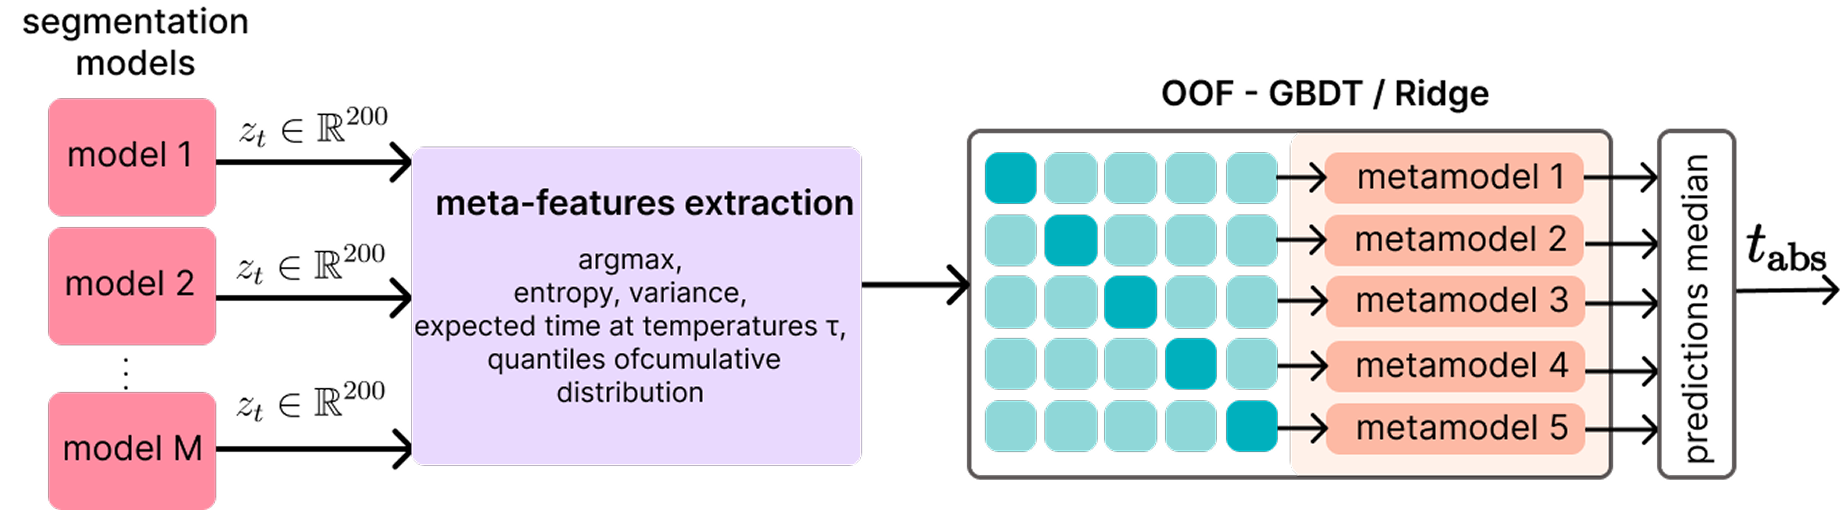
\includegraphics[width=0.9\linewidth]{img/ch1/Ch1_stacking.png}
    \caption{OOF stacking for RT prediction from time-distribution outputs. Per-model logits/distributions are converted into
    meta-features (e.g., peak time, entropy/variance, temperature-conditioned expected times, and CDF quantiles) and combined
    by a second-stage stacker (Ridge/GBDT). Predictions from fold-trained stackers are aggregated at inference (median) to produce the final RT estimate.}
    \label{fig:Ch1_stacking}
\end{figure}

\paragraph{Meta-features from logits and temperature-scaled probabilities.}
Meta-features are extracted per model from (i) raw logits and (ii) temperature-scaled probabilities computed for multiple
temperatures $\tau\in\mathcal{T}_{\text{meta}}$. From logits, a hard-peak estimate and confidence proxies are computed:

\begin{equation}
\label{eq:rt_stacking_logit_features}
t^\star = \arg\max_{t} z_t,\qquad
\hat t_{\mathrm{hard}} = t_0 + g_{t^\star},\qquad
z_{\max} = \max_t z_t,\qquad
m_{\mathrm{top2}} = z_{\max} - \max_{t\neq t^\star} z_t.
\end{equation}
For each $\tau\in\mathcal{T}_{\text{meta}}$, probabilities are formed as $p(\tau)=\mathrm{softmax}(\mathbf{z}/\tau)$ (Eq.~\ref{eq:rt_pred_dist}, Sec.~\ref{sec:rt_segmentation}), where $\mathbf{z}=(z_0,\dots,z_{T-1})$ denotes the per-time logit vector for a given model and window. Distributional summaries
are computed, including the soft-argmax time (Eq.~\ref{eq:rt_soft_argmax}, Sec.~\ref{sec:rt_segmentation}), entropy $H(p(\tau))$, peak probability
$p_{\max}(\tau)$, time variance $\mathrm{Var}_{p(\tau)}[g]$, and CDF time-quantiles (10/50/90\%). In our implementation,
$\mathcal{T}_{\text{meta}}=\{0.7,1.0,1.3\}$.

\paragraph{Meta-learner and inference.}
We use linear Ridge regression as a strong baseline meta-learner, and gradient boosting to capture non-linear reliability
patterns across models and temperatures. The meta-learner is trained using subject-disjoint cross-validation: each subject is assigned to exactly one fold (Figure~\ref{fig:Ch1_stacking}). For fold $k$, the stacker is fit on the other folds and predicts RT for the held-out fold. The leakage-controlled diagnostic is the out-of-fold nRMSE from these held-out predictions. Folds are stratified to match the per-subject mean RT distribution across folds. For held-out inference, the same feature construction is applied to unseen logits; predictions from the fold-trained stackers are aggregated to obtain the final RT estimate.
Manual blending serves as a reference, but it cannot adapt weights to sample-specific confidence profiles.

\section{Original Hidden CodaBench Benchmark Results}

We report the original hidden-release CodaBench evaluation as historical challenge context. These scores provide continuity with the original benchmark setting, while the main empirical conclusions in this manuscript are based on the labeled R11 release with subject-bootstrap confidence intervals.

\begin{table}[!h]
\centering
\caption{Original hidden-release CodaBench RT results from the earlier submission-oriented pipeline. These results are reported for historical comparison with the challenge setting.}
\label{tab:appendix_codabench}
\small
\setlength{\tabcolsep}{8pt}
\renewcommand{\arraystretch}{1.15}
\begin{tabular}{lcc}
\toprule
\textbf{Method} & \textbf{Validation nRMSE} $\downarrow$ & \textbf{Hidden nRMSE} $\downarrow$ \\
\midrule
Best temperature-tuned single model & 0.898757 & 0.92334 \\
Manual blending & 0.899979 & 0.91840 \\
Ridge stacking & 0.890430 & 0.91539 \\
Gradient boosting stacking & \textbf{0.883365} & \textbf{0.91394} \\
\bottomrule
\end{tabular}
\end{table}

\section{Unwrapped External Backbone Sanity Checks}

Unwrapped external architectures are useful for diagnosing scale sensitivity. Because our own models use per-window standardization, the primary comparison uses wrapped external models. Table~\ref{tab:appendix_unwrapped_external} reports matched sanity checks for representative off-the-shelf architectures with and without the fixed per-window standardization wrapper. The unwrapped rows often collapse toward target-standard-deviation behavior (nRMSE near 1), whereas the wrapped variants train meaningfully under the same release-separated protocol used in the main tables.

\begin{table}[!t]
\centering
\caption{Unwrapped external-backbone sanity checks. ``Wrapped'' means that the model receives the same per-window channel standardization used by our compact baselines. Lower nRMSE is better. These checks diagnose scale sensitivity; the wrapped variants are the fair external comparisons used in the main results.}
\label{tab:appendix_unwrapped_external}
\scriptsize
\setlength{\tabcolsep}{3pt}
\renewcommand{\arraystretch}{1.12}
\resizebox{\linewidth}{!}{%
\begin{tabular}{@{} l c c c c l @{}}
\toprule
\textbf{Architecture} & \textbf{Unwrapped valid} & \textbf{Unwrapped R11} & \textbf{Wrapped valid} & \textbf{Wrapped R11} & \textbf{Takeaway} \\
\midrule
EEGNet & 1.000000 & 1.002046 [0.999718, 1.007253] & 0.957877 & 0.965041 [0.954684, 0.977111] & Standardization makes the compact EEG baseline train \\
EEGConformer & 1.000000 & 1.000413 [0.999906, 1.003179] & 0.957968 & 0.962802 [0.951634, 0.975382] & Transformer-style baseline is scale-sensitive without wrapping \\
LaBraM & 1.000000 & 1.000711 [0.998638, 1.004512] & 0.958254 & 0.965382 [0.952576, 0.979330] & From-scratch foundation-style architecture needs the fixed normalization \\
\bottomrule
\end{tabular}%
}
\end{table}

\section{Additional Protocol Calibration Runs}

Protocol calibration evaluated optimizer choice, learning rate, soft-label width, batch size, and augmentation strength before fixing the training recipe used in the release-separated experiments. These diagnostics informed the protocol but are separated from the R11 results used for the main claims.

\section{Additional EventNLL Kernel and Hazard Robustness Checks}

The main text keeps the event-time segmentation table focused on the core CE, EventNLL, and control objectives, plus two compact EventNLL-family extensions. Table~\ref{tab:appendix_kernel_hazard_robustness} reports the broader kernel and hazard robustness checks. These runs use the same release-separated protocol and test whether the probabilistic event-time result depends on one specific Gaussian observation kernel or one specific softmax parameterization.

\begin{table}[!t]
\centering
\caption{Additional EventNLL kernel and hazard robustness checks. Lower nRMSE is better. ``Cal.'' denotes post-hoc temperature selection on R9--R10; the heteroscedastic run is reported at its base readout because it was not part of the calibrated kernel table.}
\label{tab:appendix_kernel_hazard_robustness}
\scriptsize
\setlength{\tabcolsep}{3pt}
\renewcommand{\arraystretch}{1.12}
\resizebox{\linewidth}{!}{%
\begin{tabular}{@{} l l c c c l @{}}
\toprule
\textbf{Variant} & \textbf{Change tested} & $\boldsymbol{\tau}$ & \textbf{Valid nRMSE} $\downarrow$ & \textbf{R11 nRMSE} $\downarrow$ & \textbf{Takeaway} \\
\midrule
Gaussian EventNLL, cal. & fixed Gaussian observation kernel & 0.70 & 0.923619 & 0.940947 [0.923160, 0.960322] & Core latent event-time likelihood reference \\
Gaussian mixture EventNLL, cal. & narrow/wide Gaussian observation mixture & 0.75 & 0.921676 & 0.939267 [0.921864, 0.958291] & Strongest calibrated EventNLL-family scalar readout \\
Laplace EventNLL, cal. & Laplace observation kernel & 0.75 & 0.926636 & 0.940696 [0.923718, 0.959285] & Robust kernel did not improve over cleaner Gaussian/mixture variants \\
Student-$t$ EventNLL, cal. & heavy-tailed Student-$t$ observation kernel & 0.80 & 0.923259 & 0.941127 [0.923382, 0.960687] & Calibration recovers validation gap, but R11 remains tied or weaker \\
Heteroscedastic EventNLL & trial-wise learned observation scale $\sigma(x)$ & 0.65 & 0.923056 & 0.942343 [0.923630, 0.962703] & Learned scale did not improve R11 enough for the core table \\
Hazard EventNLL & hazard posterior with continuous Gaussian EventNLL & 0.65 & 0.924318 & 0.937332 [0.920594, 0.955704] & Strong alternative posterior parameterization \\
Hazard discrete NLL & exact-bin discrete survival likelihood & 0.65 & 0.926288 & 0.946823 [0.928204, 0.967220] & Negative control: exact-bin survival loss is weaker than continuous EventNLL \\
\bottomrule
\end{tabular}%
}
\end{table}

Overall, these checks support two points. First, the latent event-time view is not tied to a single Gaussian-softmax implementation: the hazard EventNLL and Gaussian-mixture kernel remain competitive. Second, more robust or more flexible observation models are not automatically better; Laplace, Student-$t$, heteroscedastic, and exact-bin hazard variants are useful robustness probes but do not strengthen the core R11 story enough to feature in the main table.

\section{Additional Architecture Ablations}

Architecture ablations separate formulation effects from capacity and backbone-specific effects. In particular, ETS-U-Net capacity variants, attention bottlenecks, factorized channel interactions, recurrent variants, and EEG-Inception-style segmentation provide complementary checks on whether the event-time formulation depends on a single encoder-decoder instantiation.

\section{Additional Posterior Geometry Examples}

Table~\ref{tab:posterior_geometry_metrics} reports the quantitative posterior metrics behind Figure~\ref{fig:posterior_geometry_main}, and Figure~\ref{fig:posterior_raster_main} shows the corresponding trial-sorted posterior maps in the main text. Figure~\ref{fig:appendix_representative_posteriors} shows representative trials where models have similar scalar predictions but different posterior widths, large mode-mean gaps, or strong disagreement across losses, and Figure~\ref{fig:appendix_temperature_sensitivity} shows the development-split temperature curves used to choose post-hoc readout temperatures.

\begin{figure}[!t]
    \centering
    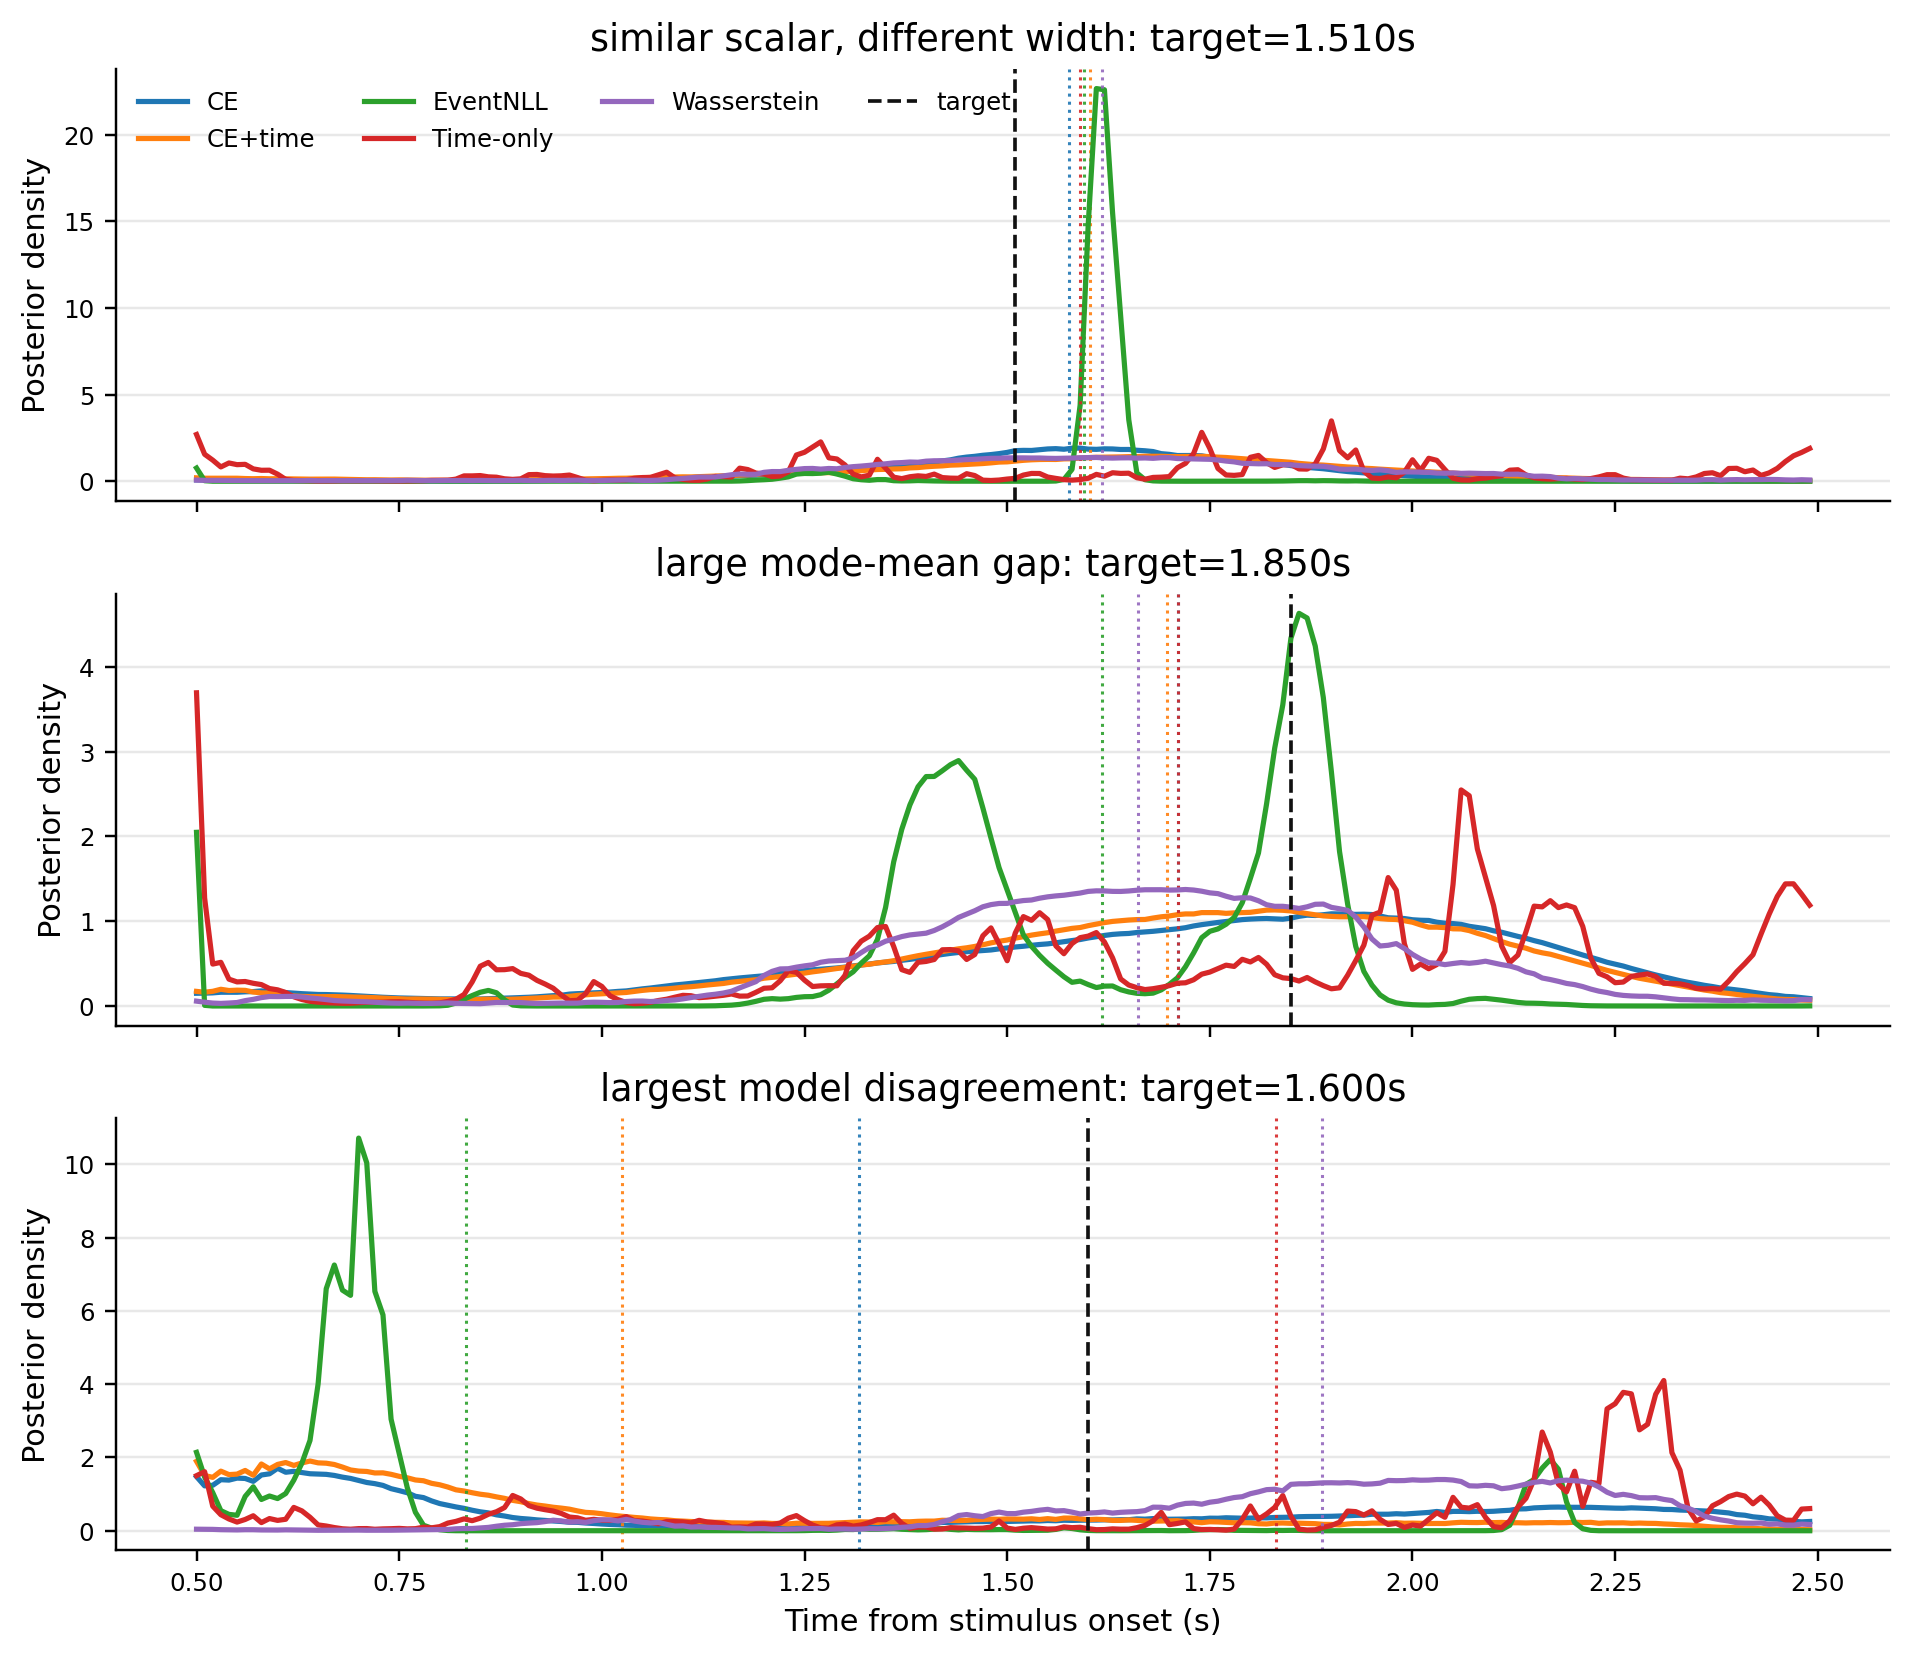
\includegraphics[width=\linewidth]{img/ch1/posterior_geometry_examples_calibrated.png}
    \caption{Representative calibrated event-time posteriors. Dashed black lines denote the true RT, and dotted colored lines denote model-specific posterior means. The examples illustrate why scalar RT alone is insufficient: models can agree on the mean while assigning very different posterior width, or disagree strongly because the posterior is multimodal or skewed.}
    \label{fig:appendix_representative_posteriors}
\end{figure}

\begin{figure}[!t]
    \centering
    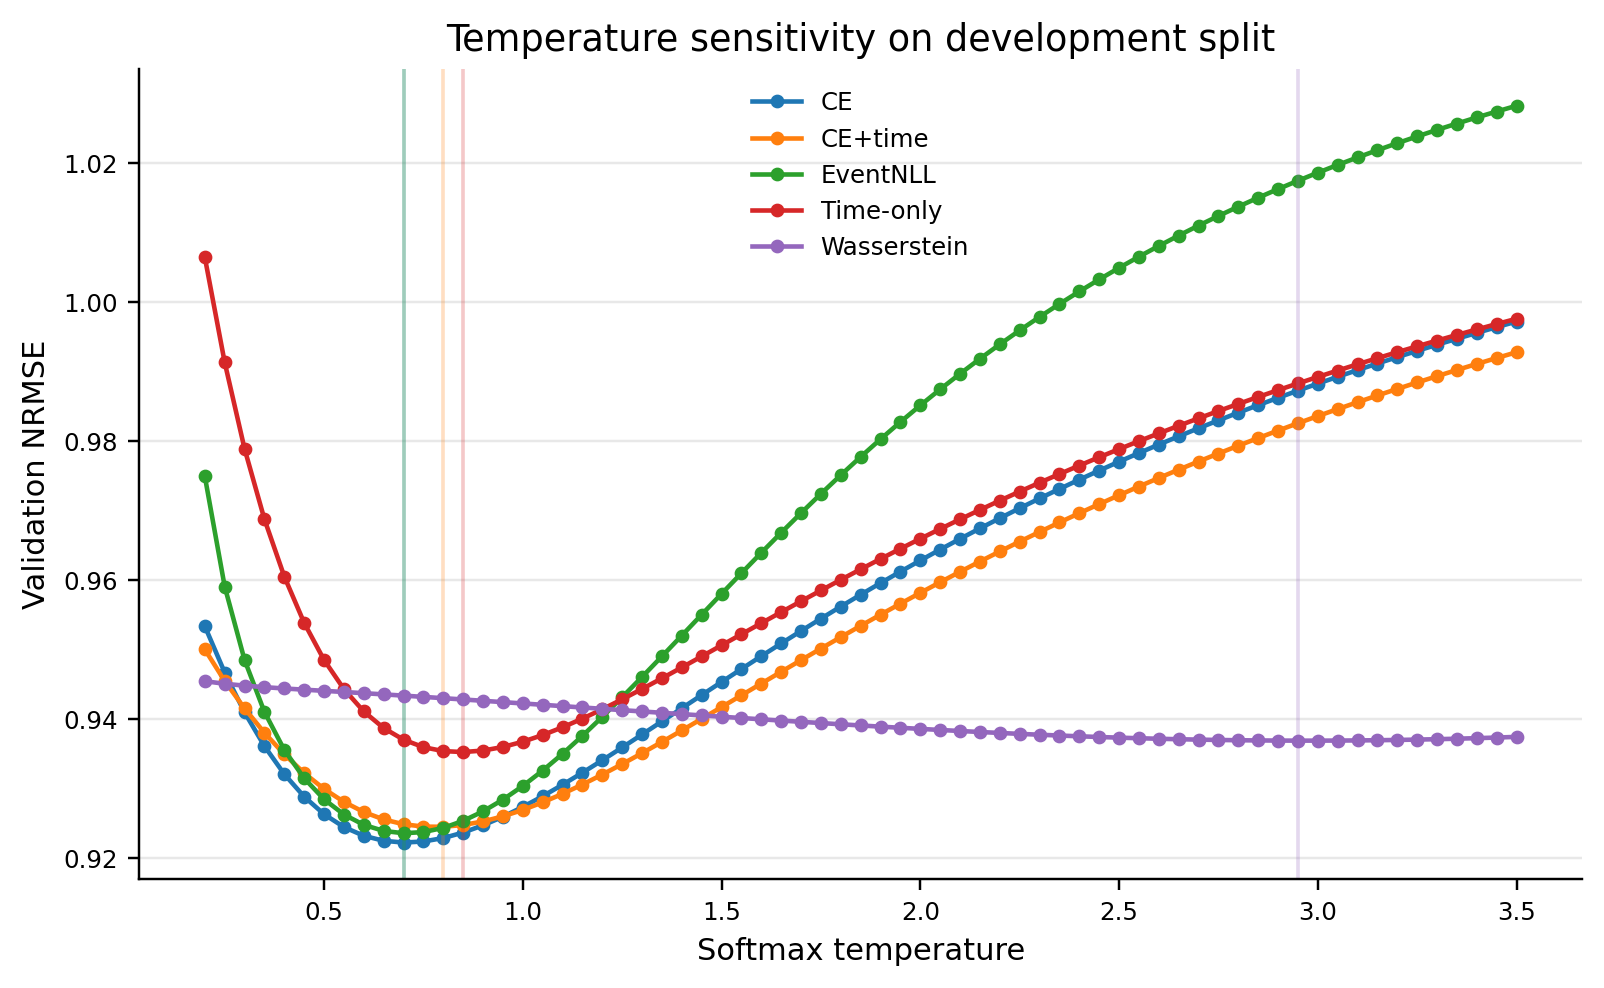
\includegraphics[width=0.9\linewidth]{img/ch1/temperature_sensitivity_calibrated.png}
    \caption{Temperature sensitivity on the R9-R10 development split. Vertical lines mark selected temperatures. The curves show that different losses induce different confidence scales, motivating temperature calibration as posterior-geometry control before comparing scalar readouts or using posterior features downstream.}
    \label{fig:appendix_temperature_sensitivity}
\end{figure}


\FloatBarrier
\clearpage
\bibliography{../references}






% \bibliographystyle{APA}
% \begin{thebibliography}{100}
% \providecommand{\natexlab}[1]{#1}
% \expandafter\ifx\csname urlstyle\endcsname\relax
%   \providecommand{\doi}[1]{doi:\discretionary{}{}{}#1}\else
%   \providecommand{\doi}{doi:\discretionary{}{}{}\begingroup
%   \urlstyle{rm}\Url}\fi

% \bibitem[{LastName(2009)}]{Ref2009}
% LastName, A. (2009).
% \newblock Title for the first reference.
% \newblock \emph{Journal of the first reference}, \emph{3}, 18 -- 88.


% \bibitem[{Authors et~al.(2008)Author1, Author2, \&
%   Author3}]{Ref2008}
% Author1, A., Author2, A., \& Author3, A. (2008).
% \newblock Title for the second reference.
% \newblock \emph{Journal for the second reference}, \emph{5}, 188 -- 200.

% \end{thebibliography}
\end{document}
